\documentclass[aspectratio=169,11pt]{beamer}
% ==========================================================================
%  KSA lecture-slide theme  =  stock beamer "Boadilla"  +  KSA colour theme
%  brand colours sampled from the official KSA symbol mark:
%    Deep Prussian Blue  #2E3192   (지성 - intellect)
%    Golden Gray         #D6CBB1   (감성 - sensibility)
%  Engine: XeLaTeX.  Usage:
%    \documentclass[aspectratio=169,11pt]{beamer}
%    % ==========================================================================
%  KSA lecture-slide theme  =  stock beamer "Boadilla"  +  KSA colour theme
%  brand colours sampled from the official KSA symbol mark:
%    Deep Prussian Blue  #2E3192   (지성 - intellect)
%    Golden Gray         #D6CBB1   (감성 - sensibility)
%  Engine: XeLaTeX.  Usage:
%    \documentclass[aspectratio=169,11pt]{beamer}
%    % ==========================================================================
%  KSA lecture-slide theme  =  stock beamer "Boadilla"  +  KSA colour theme
%  brand colours sampled from the official KSA symbol mark:
%    Deep Prussian Blue  #2E3192   (지성 - intellect)
%    Golden Gray         #D6CBB1   (감성 - sensibility)
%  Engine: XeLaTeX.  Usage:
%    \documentclass[aspectratio=169,11pt]{beamer}
%    \input{../theme/ksa-theme.tex}
% ==========================================================================

\usepackage{fontspec}
\usepackage{amsmath,amssymb}
\usepackage{graphicx}
\graphicspath{{figs/}{../figs/}}
\usepackage{booktabs}
\usepackage{listings}

% ---- fonts (no ctex/xeCJK on this box -> fontspec drives CJK directly) -----
\defaultfontfeatures{Ligatures=TeX}
\setmainfont{Noto Sans CJK KR}
\setsansfont{Noto Sans CJK KR}
\setmonofont{Noto Sans Mono CJK KR}[Scale=0.92]

% ---- base theme: stock Boadilla ------------------------------------------
\usetheme{Boadilla}
\usefonttheme{professionalfonts}
\setbeamertemplate{navigation symbols}{}

% ---- KSA colour theme (recolour the stock theme) --------------------------
\definecolor{ksablue}{HTML}{2E3192}
\definecolor{ksabluedk}{HTML}{20226A}
\definecolor{ksagold}{HTML}{D6CBB1}
\definecolor{ksagolddk}{HTML}{A9976B}
\definecolor{ksared}{HTML}{C0392B}
\definecolor{ksagray}{HTML}{5B5B5B}

\setbeamercolor{structure}{fg=ksablue}
\setbeamercolor{alerted text}{fg=ksared}

\setbeamercolor{palette primary}{fg=white,           bg=ksablue}
\setbeamercolor{palette secondary}{fg=white,         bg=ksablue!85!black}
\setbeamercolor{palette tertiary}{fg=white,          bg=ksabluedk}
\setbeamercolor{titlelike}{fg=ksablue}
\setbeamercolor{frametitle}{fg=ksablue,bg=}
\setbeamercolor{title}{fg=ksablue}
\setbeamercolor{author}{fg=ksagray}
\setbeamercolor{institute}{fg=ksagray}
\setbeamercolor{block title}{fg=white,bg=ksablue}
\setbeamercolor{block body}{fg=black!85,bg=ksablue!6}
\setbeamercolor{item}{fg=ksablue}
\setbeamercolor{section in toc}{fg=black!85}

\setbeamerfont{frametitle}{series=\bfseries}
\setbeamerfont{title}{series=\bfseries}

% ---- footline:  KSA mark | "Made by ..." | n / N   (matches reference) ----
\newcommand{\ksacredit}{Made by Sumin Han \,\textperiodcentered\, suminhan@ksa.hs.kr}
\setbeamertemplate{footline}{%
  \hbox{%
    \begin{beamercolorbox}[wd=.18\paperwidth,ht=2.6ex,dp=1.5ex,leftskip=1.1em]{}%
      \raisebox{-0.35ex}{
\includegraphics[height=2.0ex]{ksa-logo.png}}%
    \end{beamercolorbox}%
    \begin{beamercolorbox}[wd=.64\paperwidth,ht=2.6ex,dp=1.5ex,center]{}%
      {\scriptsize\color{ksagray}\ksacredit}%
    \end{beamercolorbox}%
    \begin{beamercolorbox}[wd=.18\paperwidth,ht=2.6ex,dp=1.5ex,rightskip=1.1em]{}%
      \hfill{\scriptsize\color{ksablue}\insertframenumber\,/\,\inserttotalframenumber}%
    \end{beamercolorbox}%
  }%
  \vskip2pt
}

% ---- section divider: stock \sectionpage, KSA-coloured -------------------
\setbeamertemplate{section page}{%
  \begingroup\centering
    {\color{ksagolddk}\rule{0.16\paperwidth}{1pt}}\par\vskip1.0em
    {\usebeamerfont{title}\color{ksablue}\insertsectionhead\par}\vskip1.0em
    {\color{ksagolddk}\rule{0.16\paperwidth}{1pt}}\par
  \endgroup
}
\AtBeginSection[]{\begin{frame}[plain,noframenumbering]\vfill\sectionpage\vfill\end{frame}}

% ---- code listings ------------------------------------------------------------
\lstdefinestyle{ksa}{%
  basicstyle=\ttfamily\scriptsize,
  keywordstyle=\color{ksablue}\bfseries,
  commentstyle=\color{ksagray}\itshape,
  stringstyle=\color{ksagolddk},
  numberstyle=\tiny\color{ksagray},
  backgroundcolor=\color{ksablue!6},
  frame=leftline, framerule=1.4pt, rulecolor=\color{ksablue},
  xleftmargin=1em, aboveskip=0.8em, belowskip=0.4em,
  showstringspaces=false, breaklines=true, language=Python,
}
\lstset{style=ksa}

% ---- handy macros -----------------------------------------------------------
\newcommand{\kb}[1]{\textbf{\color{ksablue}#1}}   % blue keyword
\newcommand{\kq}[1]{\textbf{\color{ksared}#1}}    % red key-question

% ==========================================================================

\usepackage{fontspec}
\usepackage{amsmath,amssymb}
\usepackage{graphicx}
\graphicspath{{figs/}{../figs/}}
\usepackage{booktabs}
\usepackage{listings}

% ---- fonts (no ctex/xeCJK on this box -> fontspec drives CJK directly) -----
\defaultfontfeatures{Ligatures=TeX}
\setmainfont{Noto Sans CJK KR}
\setsansfont{Noto Sans CJK KR}
\setmonofont{Noto Sans Mono CJK KR}[Scale=0.92]

% ---- base theme: stock Boadilla ------------------------------------------
\usetheme{Boadilla}
\usefonttheme{professionalfonts}
\setbeamertemplate{navigation symbols}{}

% ---- KSA colour theme (recolour the stock theme) --------------------------
\definecolor{ksablue}{HTML}{2E3192}
\definecolor{ksabluedk}{HTML}{20226A}
\definecolor{ksagold}{HTML}{D6CBB1}
\definecolor{ksagolddk}{HTML}{A9976B}
\definecolor{ksared}{HTML}{C0392B}
\definecolor{ksagray}{HTML}{5B5B5B}

\setbeamercolor{structure}{fg=ksablue}
\setbeamercolor{alerted text}{fg=ksared}

\setbeamercolor{palette primary}{fg=white,           bg=ksablue}
\setbeamercolor{palette secondary}{fg=white,         bg=ksablue!85!black}
\setbeamercolor{palette tertiary}{fg=white,          bg=ksabluedk}
\setbeamercolor{titlelike}{fg=ksablue}
\setbeamercolor{frametitle}{fg=ksablue,bg=}
\setbeamercolor{title}{fg=ksablue}
\setbeamercolor{author}{fg=ksagray}
\setbeamercolor{institute}{fg=ksagray}
\setbeamercolor{block title}{fg=white,bg=ksablue}
\setbeamercolor{block body}{fg=black!85,bg=ksablue!6}
\setbeamercolor{item}{fg=ksablue}
\setbeamercolor{section in toc}{fg=black!85}

\setbeamerfont{frametitle}{series=\bfseries}
\setbeamerfont{title}{series=\bfseries}

% ---- footline:  KSA mark | "Made by ..." | n / N   (matches reference) ----
\newcommand{\ksacredit}{Made by Sumin Han \,\textperiodcentered\, suminhan@ksa.hs.kr}
\setbeamertemplate{footline}{%
  \hbox{%
    \begin{beamercolorbox}[wd=.18\paperwidth,ht=2.6ex,dp=1.5ex,leftskip=1.1em]{}%
      \raisebox{-0.35ex}{
\includegraphics[height=2.0ex]{ksa-logo.png}}%
    \end{beamercolorbox}%
    \begin{beamercolorbox}[wd=.64\paperwidth,ht=2.6ex,dp=1.5ex,center]{}%
      {\scriptsize\color{ksagray}\ksacredit}%
    \end{beamercolorbox}%
    \begin{beamercolorbox}[wd=.18\paperwidth,ht=2.6ex,dp=1.5ex,rightskip=1.1em]{}%
      \hfill{\scriptsize\color{ksablue}\insertframenumber\,/\,\inserttotalframenumber}%
    \end{beamercolorbox}%
  }%
  \vskip2pt
}

% ---- section divider: stock \sectionpage, KSA-coloured -------------------
\setbeamertemplate{section page}{%
  \begingroup\centering
    {\color{ksagolddk}\rule{0.16\paperwidth}{1pt}}\par\vskip1.0em
    {\usebeamerfont{title}\color{ksablue}\insertsectionhead\par}\vskip1.0em
    {\color{ksagolddk}\rule{0.16\paperwidth}{1pt}}\par
  \endgroup
}
\AtBeginSection[]{\begin{frame}[plain,noframenumbering]\vfill\sectionpage\vfill\end{frame}}

% ---- code listings ------------------------------------------------------------
\lstdefinestyle{ksa}{%
  basicstyle=\ttfamily\scriptsize,
  keywordstyle=\color{ksablue}\bfseries,
  commentstyle=\color{ksagray}\itshape,
  stringstyle=\color{ksagolddk},
  numberstyle=\tiny\color{ksagray},
  backgroundcolor=\color{ksablue!6},
  frame=leftline, framerule=1.4pt, rulecolor=\color{ksablue},
  xleftmargin=1em, aboveskip=0.8em, belowskip=0.4em,
  showstringspaces=false, breaklines=true, language=Python,
}
\lstset{style=ksa}

% ---- handy macros -----------------------------------------------------------
\newcommand{\kb}[1]{\textbf{\color{ksablue}#1}}   % blue keyword
\newcommand{\kq}[1]{\textbf{\color{ksared}#1}}    % red key-question

% ==========================================================================

\usepackage{fontspec}
\usepackage{amsmath,amssymb}
\usepackage{graphicx}
\graphicspath{{figs/}{../figs/}}
\usepackage{booktabs}
\usepackage{listings}

% ---- fonts (no ctex/xeCJK on this box -> fontspec drives CJK directly) -----
\defaultfontfeatures{Ligatures=TeX}
\setmainfont{Noto Sans CJK KR}
\setsansfont{Noto Sans CJK KR}
\setmonofont{Noto Sans Mono CJK KR}[Scale=0.92]

% ---- base theme: stock Boadilla ------------------------------------------
\usetheme{Boadilla}
\usefonttheme{professionalfonts}
\setbeamertemplate{navigation symbols}{}

% ---- KSA colour theme (recolour the stock theme) --------------------------
\definecolor{ksablue}{HTML}{2E3192}
\definecolor{ksabluedk}{HTML}{20226A}
\definecolor{ksagold}{HTML}{D6CBB1}
\definecolor{ksagolddk}{HTML}{A9976B}
\definecolor{ksared}{HTML}{C0392B}
\definecolor{ksagray}{HTML}{5B5B5B}

\setbeamercolor{structure}{fg=ksablue}
\setbeamercolor{alerted text}{fg=ksared}

\setbeamercolor{palette primary}{fg=white,           bg=ksablue}
\setbeamercolor{palette secondary}{fg=white,         bg=ksablue!85!black}
\setbeamercolor{palette tertiary}{fg=white,          bg=ksabluedk}
\setbeamercolor{titlelike}{fg=ksablue}
\setbeamercolor{frametitle}{fg=ksablue,bg=}
\setbeamercolor{title}{fg=ksablue}
\setbeamercolor{author}{fg=ksagray}
\setbeamercolor{institute}{fg=ksagray}
\setbeamercolor{block title}{fg=white,bg=ksablue}
\setbeamercolor{block body}{fg=black!85,bg=ksablue!6}
\setbeamercolor{item}{fg=ksablue}
\setbeamercolor{section in toc}{fg=black!85}

\setbeamerfont{frametitle}{series=\bfseries}
\setbeamerfont{title}{series=\bfseries}

% ---- footline:  KSA mark | "Made by ..." | n / N   (matches reference) ----
\newcommand{\ksacredit}{Made by Sumin Han \,\textperiodcentered\, suminhan@ksa.hs.kr}
\setbeamertemplate{footline}{%
  \hbox{%
    \begin{beamercolorbox}[wd=.18\paperwidth,ht=2.6ex,dp=1.5ex,leftskip=1.1em]{}%
      \raisebox{-0.35ex}{
\includegraphics[height=2.0ex]{ksa-logo.png}}%
    \end{beamercolorbox}%
    \begin{beamercolorbox}[wd=.64\paperwidth,ht=2.6ex,dp=1.5ex,center]{}%
      {\scriptsize\color{ksagray}\ksacredit}%
    \end{beamercolorbox}%
    \begin{beamercolorbox}[wd=.18\paperwidth,ht=2.6ex,dp=1.5ex,rightskip=1.1em]{}%
      \hfill{\scriptsize\color{ksablue}\insertframenumber\,/\,\inserttotalframenumber}%
    \end{beamercolorbox}%
  }%
  \vskip2pt
}

% ---- section divider: stock \sectionpage, KSA-coloured -------------------
\setbeamertemplate{section page}{%
  \begingroup\centering
    {\color{ksagolddk}\rule{0.16\paperwidth}{1pt}}\par\vskip1.0em
    {\usebeamerfont{title}\color{ksablue}\insertsectionhead\par}\vskip1.0em
    {\color{ksagolddk}\rule{0.16\paperwidth}{1pt}}\par
  \endgroup
}
\AtBeginSection[]{\begin{frame}[plain,noframenumbering]\vfill\sectionpage\vfill\end{frame}}

% ---- code listings ------------------------------------------------------------
\lstdefinestyle{ksa}{%
  basicstyle=\ttfamily\scriptsize,
  keywordstyle=\color{ksablue}\bfseries,
  commentstyle=\color{ksagray}\itshape,
  stringstyle=\color{ksagolddk},
  numberstyle=\tiny\color{ksagray},
  backgroundcolor=\color{ksablue!6},
  frame=leftline, framerule=1.4pt, rulecolor=\color{ksablue},
  xleftmargin=1em, aboveskip=0.8em, belowskip=0.4em,
  showstringspaces=false, breaklines=true, language=Python,
}
\lstset{style=ksa}

% ---- handy macros -----------------------------------------------------------
\newcommand{\kb}[1]{\textbf{\color{ksablue}#1}}   % blue keyword
\newcommand{\kq}[1]{\textbf{\color{ksared}#1}}    % red key-question


\title{Block B 캡스톤: 팀 프로젝트와 학기 총정리}
\subtitle{16.1 팀 프로젝트: 발표 \,\textperiodcentered\, 16.2 Peer-Review \,\textperiodcentered\, 16.3 ML2 총정리와 학기를 넘어서}
\author{Machine Learning 2 \,\textperiodcentered\, 16주차}
\institute{한국과학영재학교 (KSA)}
\date{Chapter 16}

\begin{document}

% ===== title =====
\begin{frame}[plain,noframenumbering]
  \titlepage
\end{frame}

% ===== roadmap of this week =====
\begin{frame}{이번 주차 개요}
  \small
  \textbf{이 챕터를 마치면}
  \begin{enumerate}
    \item 연속제어 환경에서 4주 파이프라인(환경 고르기 $\to$ 구현 $\to$ 평가
      $\to$ 발표)으로 팀 프로젝트를 설계·실행하고, ``시드 $\geq 3$ · 무작위
      정책 베이스라인 · 학습/평가 분리'' 프로토콜을 실제로 수행할 수 있다.
    \item ``학습 곡선이 올랐다''와 ``배운 정책이 무작위보다 낫다''가 서로 다른
      문장임을 구분하고, 학습 도중(탐험 포함) 성과와 학습 후 결정적($a=\mu$)
      평가의 격차를 11.2절의 분산 원리로 해석할 수 있다.
    \item 5항목 체크리스트와 1점(감상평) $\to$ 3점(반박 가능한 질문) 기준으로
      다른 팀의 발표를 심사하는 peer-review를 작성할 수 있다.
    \item 학기 전체를 ``모델 정의 $\to$ 틀린 정도를 수치화 $\to$ 개선'' 3단계로
      정리하고, 학기 이후 방향(오프라인 RL · 범용 로봇 정책 · sim-to-real)을
      자기 언어로 말할 수 있다.
  \end{enumerate}
  \vskip0.5em
  \begin{itemize}
    \item \kb{16.1} 팀 프로젝트: 발표 — Pendulum 실습, 시드 3개, 결정적 평가, 4주 파이프라인
    \item \kb{16.2} Peer-Review — 이번엔 네가 심사위원. ``우연히 좋은'' 패턴 5가지
    \item \kb{16.3} ML2 총정리 — 하나의 MDP를 네 경로로, 20문항 자가진단, 최신 동향
  \end{itemize}
  \vskip0.4em
  \kq{Ch.\,9--15로 새 도구(신경망·시뮬레이션·트리 탐색)를 다 갖췄다.
  이 장부터는 배울 개념이 남지 않는다 — 도구를 로봇 시뮬레이션에 직접
  적용해, 그 결과를 정직하게 보고하는 것으로 학기를 마무리한다.}
\end{frame}

\section{16.1 팀 프로젝트: 발표}

\begin{frame}{왜 지금 프로젝트를 하는가 — Chapter 8의 쌍(pair)}
  \begin{itemize}
    \item 8.1 Block A 캡스톤: ``코드가 동작한다'' vs. ``내가 문제를 설계하고
      평가할 수 있다''의 차이에 대한 첫 답.
    \item Ch.\,9--15가 두 번째 절반의 도구를 전부 줬다: 표 대신
      \textbf{신경망(DQN)}, 정책을 직접 학습(REINFORCE·PPO), 시연·선호로부터
      배우기(모방학습), 물리 시뮬레이션(MuJoCo·Isaac Sim), 트리 탐색(MCTS).
    \item \kb{16.1 = Chapter 8과 쌍인 절} — 같은 절차(환경 고르기 $\to$ 구현
      $\to$ 시드 프로토콜 $\to$ 수식적 정당화 $\to$ 정직한 발표)를
      \textbf{완전히 다른 무대}(연속제어 + 신경망)에서 다시 집행.
  \end{itemize}
  \vskip0.5em
  \small
  \begin{tabular}{@{}lll@{}}
    \toprule
     & Block A (8.1) & Block B (이 절) \\
    \midrule
    환경 & 표 기반(이산 상태·행동) & 연속제어(연속 상태·행동) \\
    알고리즘 & 2개 이상(Q-learning vs SARSA) & 1개 이상(DQN/PPO/모방/MCTS) \\
    평가 프로토콜 & $\varepsilon=0$(greedy) 에피소드 & 결정적 실행 $a=\mu$ 에피소드 \\
    1시드 예산 & 초$\sim$분 단위 & Pendulum 12만 스텝 $\approx$20$\sim$30초 $\sim$ MuJoCo 시간 단위 \\
    시드 $\geq 3$ · 베이스라인 & 동일 & 동일 \\
    \bottomrule
  \end{tabular}
\end{frame}

\begin{frame}{왜 알고리즘은 ``1개 이상''인가}
  \begin{itemize}
    \item Block A: 두 번째 알고리즘은 \textbf{갱신 규칙 한 줄의 차이}(6.3) —
      Q-learning vs SARSA.
    \item Block B: 각 알고리즘이 \textbf{별개의 신경망 학습 파이프라인}.
      \begin{itemize}
        \item DQN: 리플레이 버퍼 + 타깃 네트워크가 따라온다.
        \item PPO: GAE + 클리핑이 따라온다.
        \item 모방학습: 시연 데이터셋이 따라온다.
      \end{itemize}
    \item 팀 단위 현실적 예산: ``한 파이프라인을 제대로 돌리고, 여유가
      있으면 비교''.
  \end{itemize}
  \vskip0.6em
  \begin{block}{변하지 않는 것이 핵심}
    시드 $\geq 3$ · 베이스라인(무작위 정책) · 학습/평가 분리는 알고리즘과
    무관한 \textbf{강화학습 실험의 골격}이라 Block A와 동일하다.
  \end{block}
\end{frame}

\begin{frame}{역사: 왜 Pendulum인가}
  \begin{itemize}
    \item OpenAI 생태계(baselines $\to$ stable-baselines) 시대부터 연속 제어의
      ``hello world'' — 라이브러리 PPO 튜토리얼의 표준 예제.
    \item PPO 논문(Schulman et al., 2017)은 같은 계열의 MuJoCo 연속 제어
      고전 과제(Swimmer, Hopper 등)에서 검증.
    \item Pendulum은 그중 \textbf{가장 작은} 구성원: 3차원 상태, 1차원 행동,
      에피소드 종료도 목표 상태도 없음 — ``매 스텝 균형을 해야 하는''
      보상이 연속 제어의 본질적 어려움을 최소 분량에 담는다.
  \end{itemize}
  \vskip0.6em
  \kq{첫 과제로 고르는 이유는 ``쉬워서''가 아니라, 그 보상 구조가
  학습 곡선 위에서 ``정책이 지금 무엇을 하고 있는지''를 가장 선명하게
  보여주기 때문이다.}
\end{frame}

\begin{frame}{프로젝트 구조 — 환경 · 적용 · 필수 요구사항}
  \begin{itemize}
    \item \textbf{환경}: PyBullet 또는 Gymnasium의 연속제어 환경
      (Pendulum, MuJoCo 기반 로봇 등) 중 하나.
    \item \textbf{적용}: Chapter 9--15 중 \textbf{최소 하나의 방법}(DQN, PPO,
      모방학습, MCTS)으로 정책을 학습.
    \item \textbf{필수 — 수식적 정당화 최소 1개}, 예:
      \begin{itemize}
        \item PPO: Ch11.3의 클리핑이 학습 안정성에 미친 영향(있음/없음 비교)
        \item 모방학습: Ch12.1의 복합 오차 관찰(전문가 데이터 분포 밖 성능 저하)
        \item 도메인 무작위화: Ch13.1의 현실 격차 논의와 연결해 효과 설명
      \end{itemize}
    \item \kb{학습 곡선(에피소드별 누적 보상)은 반드시 제시} — 지도학습의
      손실 곡선에 해당하는, ``학습이 실제로 되고 있는가''의 기본 증거.
  \end{itemize}
\end{frame}

\begin{frame}{환경 고르는 실전 가이드 — 후보에 점수를 매기자}
  \small
  \begin{enumerate}
    \item \textbf{상태·행동 공간의 차원} — 차원이 높으면 학습 예산이
      급격히 커짐(예: HumanoidStandup은 $348\times17$).
    \item \textbf{보상 구조} — ``항상 음수(0이 목표)''형(Pendulum)과
      ``희소(목표 도달 시에만)''형(13.1 Reacher)은 \textbf{좋은 정책의
      모습} 자체가 달라 평가 지표의 의미가 달라진다.
    \item \textbf{시뮬레이션 격차가 보일 만큼 물리적으로 풍부한가} —
      13.1 도메인 무작위화를 제시하려면 Pendulum은 격차가 안 나와
      MuJoCo 로봇이 적합.
    \item \textbf{코드 재사용성} — Ch11.2의 PPO 코드가 거의 그대로
      적용되는가.
  \end{enumerate}
  \vskip0.5em
  \begin{block}{왜 점수 매기기를 하는가}
    기준을 먼저 정해두면 \textbf{팀 회의가 쉬워진다}(8.1절의 방식 그대로).
    환경은 ``임의로 고르는'' 것이 아니라 기준에 대해 점수를 받는 것.
  \end{block}
\end{frame}

\begin{frame}{환경 후보 비교 — Block B 대표 4종}
  \small
  \begin{tabular}{@{}lllll@{}}
    \toprule
    환경 & 상태$\times$행동 & 보상 구조 & 에피소드 & 잘 어울리는 비교/개념 \\
    \midrule
    \textbf{Pendulum-v1} & 3$\times$1 (연속) & $r=-\theta^2-0.1\dot\theta^2-0.001a^2$, 항상 음수(0=완벽) & 200 & PPO(Ch11) 클래식 페어링 — 클리핑 효과(11.3) \\
    \textbf{CartPole-v1} & 4$\times$2 (이산) & 생존 시 스텝당 $-1$, 쓰러지면 종료 & 500 & DQN(Ch9) vs PPO — 이산 행동·연속 상태 \\
    \textbf{MountainCar-v0} & 2$\times$3 (이산) & 스텝당 $-1$ (희소) & 200 & 희소 보상 + 긴 지평 — GAE $\lambda$ 트레이드오프(11.3) \\
    \textbf{HumanoidStandup-v5} & 348$\times$17 (연속) & 포텐셜 기반 shaping(Ch14) & 1000 & 도메인 무작위화(13.1), MuJoCo 경험(Ch14) \\
    \bottomrule
  \end{tabular}
  \vskip1em
  {\footnotesize 보상 구조의 ``형''이 다르면 좋은 정책의 \textbf{모습} 자체가 달라
  --- 평가 지표의 의미가 바뀐다.}
\end{frame}

\begin{frame}{환경-알고리즘 ``페어링'' 논리}
  \begin{itemize}
    \item ``잘 어울리는'' 열의 논리가 핵심 — \kb{환경과 알고리즘은
      ``검증하고 싶은 개념이 돋보이는 무대''가 무엇인가를 기준으로
      짝을 이루어 골라야 한다}.
    \item 11.3의 클리핑(있음/없음)을 발표하고 싶으면 $\to$ 연속 행동 공간에서
      클리핑이 실제로 발동하는 \textbf{Pendulum}.
    \item 13.1의 도메인 무작위화를 발표하고 싶으면 $\to$ 격차가 생길 만큼
      물리적으로 풍부한 \textbf{MuJoCo} 환경.
    \item 12.1의 복합 오차를 발표하고 싶으면 $\to$ \textbf{전문가 시연
      데이터셋}이 있는 모방학습 과제.
  \end{itemize}
  \vskip0.6em
  \begin{center}
    \kq{``PPO를 쓰고 싶은데 환경을 뭐로 하지?''는 순서가 틀린 질문.\\
    ``개념 X를 테스트하고 싶은데 무대는 어디인가?''가 올바른 질문이다.}
  \end{center}
\end{frame}

\begin{frame}{베이스라인: 무작위 정책의 리턴을 먼저 재자}
  \begin{itemize}
    \item M1 제출물의 핵심 숫자 — ``배운 정책이 실제로 \textbf{무작위보다
      나은가}''를 판정할 \kb{제로점}이 없으면 ``개선됐다''고 말할 수 없다.
    \item Pendulum-v1 매 스텝 무작위 토크 정책(100 에피소드)의 평균 리턴:
      \textbf{$-1274.1$ (sd 300.0)}, 대략 $[-1800,\,-760]$ 구간에 분포.
    \item \textbf{읽기 1} — ``0''과 ``좋음''의 거리가 표 기반보다 훨씬 크다.
      CliffWalking은 무작위 $-5000 \to$ 학습 후 $-13$ (400배 격차)였는데,
      여기선 ``좋음''이 0이고 무작위가 이미 $-1274$ — \textbf{0까지의 거리
      자체가 지표}.
    \item \textbf{읽기 2} — 아무것도 하지 않는 정책이 생각보다 나쁘지 않다.
      토크 0 고정(zero-torque)이 약 \textbf{$-1230$}으로 무작위와 같은 등급.
    \item ``학습 곡선이 $-1200$ 부근에서 시작한다''는 사실은 \textbf{학습의
      증거가 전혀 안 된다} — 이 두 숫자(무작위 $-1274$, zero-torque $-1230$)를
      먼저 재야 ``PPO가 $-673$(무작위의 절반)''이라는 판단이 성립한다.
  \end{itemize}
\end{frame}

\begin{frame}{비교 프로토콜: 연속제어 버전 3개 항목}
  8.1절 프로토콜(시드 $\geq 3$, 학습 중/학습 후 분리, 시드별 표)을 연속제어로
  번역 — 1·3은 그대로, \textbf{두 번째가 번역된다}.
  \vskip0.6em
  \begin{enumerate}
    \item \textbf{학습 시드 $\geq 3$개} — 시드를 바꾸는 것은 ``실험을 다시
      하는'' 것이 아니라 \textbf{``우연인지 재검사하는''} 것. PPO는
      초기화·샘플링·데이터 분할의 무작위성이 겹쳐 같은 코드도 시드만 바꿔도
      곡선 모양이 달라짐 (11.2: 큰 그림은 시드마다 안정적이나 마지막
      10에피소드 평균은 $\pm100\sim200$ 흔들림).
    \item \textbf{학습 도중 성과 vs 학습 후 평가} — $\varepsilon=0$의
      ``번역 문제'' (다음 프레임).
    \item \textbf{알고리즘/시드별 숫자를 표로 제시}.
  \end{enumerate}
  \vskip0.4em
  {\footnotesize 표 기반 $\varepsilon$-greedy에는 깔끔한 핸들이 있었음:
  평가 때 $\varepsilon=0$으로 하면 ``순수 탐욕적''. 연속 정책
  $a\sim\mathcal{N}(\mu_\theta(s),\,\sigma_\theta^2)$에는
  $\varepsilon$이라는 핸들이 \textbf{없다}.}
\end{frame}

\begin{frame}{$\varepsilon=0$의 대응물 — 왜 $a=\mu$인가}
  \begin{columns}[T]
    \begin{column}{0.55\textwidth}
      \textbf{대응 원리}
      \begin{itemize}
        \item \textbf{학습 도중(샘플) 평가}: 학습 중과 같은 $a=\mu+\sigma z$로
          실행 — \textbf{탐험 노이즈가 섞인} 성과.
        \item \textbf{학습 후(결정적) 평가}: $a=\mu_\theta(s)$만 내보내고
          샘플링 안 함 — \textbf{연속제어의 ``greedy 평가'' 대응물}.
      \end{itemize}
      \vskip0.4em
      \kb{왜 $a=\mu$가 $\varepsilon=0$인가?}
      \begin{itemize}
        \item $\varepsilon$-greedy에서 $\varepsilon$의 역할 = ``확률
          $\varepsilon$로 아무 행동이나''.
        \item 정규분포 정책에서 ``아무 행동''에 해당하는 것은 \textbf{샘플링
          노이즈 $z$} — 빼면 ``정책의 최선 추측'' $\mu$만 남는다.
      \end{itemize}
    \end{column}
    \begin{column}{0.42\textwidth}
      \begin{block}{$\sigma$를 0으로 만들면 안 되는 이유}
        $\sigma$는 \textbf{학습된 파라미터} — 11.2의 엔트로피 보너스가
        0으로 쪼그라들지 않게 브레이크 역할.\\
        평가 때 $\sigma=0$으로 ``학습''하는 것이 아니라,
        \textbf{파라미터를 그대로 두고 샘플링만 하지 않는 것}이 정직한
        ``탐험 제거''.
        {\footnotesize (``$\sigma$를 0으로 설정해서 돌려라''는 오답 —
        파라미터를 바꾼 \emph{다른} 정책의 실행이 되기 때문.)}
      \end{block}
    \end{column}
  \end{columns}
\end{frame}

\begin{frame}{실측: 3시드 결과 표와 읽기 1·2}
  {\footnotesize 실습 노트북: Ch11.2의 PPO 그대로, $\gamma=0.99$,
  $\lambda=0.95$, $\epsilon_{\text{clip}}=0.2$, lr=3e-4, 시드당
  300반복$\times$400스텝 = 12만 스텝, 시드 0/1/2, 평가 50 에피소드}
  \vskip0.6em
  \small
  \begin{tabular}{@{}llll@{}}
    \toprule
    시드 & 학습 도중 마지막10 & 학습 후 결정적 $a=\mu$ & 학습 후 샘플 $a\sim\mathcal{N}$ \\
    \midrule
    0 & $-673.5$ & $-1357.9$ & $-1287.6$ \\
    1 & $-732.3$ & $-1454.2$ & $-1399.4$ \\
    2 & $-668.3$ & $-1398.2$ & $-1367.0$ \\
    (베이스라인) & --- & --- & 무작위 $-1274.1$ (100 에피소드) \\
    \bottomrule
  \end{tabular}
  \vskip0.8em
  이 표는 \textbf{세 번} 읽어야 하고, 세 번째가 이 절의 핵심이다.
  \begin{itemize}
    \item \textbf{읽기 1 — 학습 도중 곡선은 정말 올랐다}: 마지막 10
      ($-673/-732/-668$)이 첫 10 ($-777/-866/-914$) 대비 \textbf{15$\sim$27\%
      개선}, 무작위 $-1274$보다 대략 2배 낫다. 이 숫자만 보면 ``학습 성공''.
    \item \textbf{읽기 2 — 시드 간 편차가 있지만 방향은 일관}: 마지막 10의
      시드 간 격차 약 65 ($-668\sim-732$)로 ``같은 모양'' 범위 — 11.2의
      ``큰 그림은 시드마다 안정적''이 재현된다.
  \end{itemize}
\end{frame}

\begin{frame}{읽기 3 — 결정적 평가가 베이스라인 \emph{아래}다}
  \begin{columns}[T]
    \begin{column}{0.55\textwidth}
      \begin{itemize}
        \item 세 시드의 $a=\mu$ 평가 평균 $\approx$ \textbf{$-1403$}으로
          무작위 정책 ($-1274$) \textbf{아래}.
      \end{itemize}
      \vskip0.3em
      \begin{center}
      \kq{``학습 곡선이 올랐다''와 ``배운 정책이 무작위보다 낫다''는\\
      서로 다른 두 문장이다.}
      \end{center}
      \begin{itemize}
        \item 왜? 학습 도중 리턴은 \textbf{탐험 노이즈 $\sigma$가 섞인 채}
          측정한 것 — $\sigma$ 샘플링이 운 좋게 진자를 높이 스윙하게 한
          에피소드가 평균에 들어감 (11.2 FAQ: ``에피소드 리턴 \emph{자체}의
          분산은 줄일 수 없다'').
        \item 노이즈를 빼면 12만 스텝으로는 $\mu$가 상태별로 아직 정확하지
          못해, 결정적 정책은 ``대충 그럴듯한 범위로 스윙'' 수준
          (아무것도 안 함 $\approx -1230$과 같은 등급).
        \item \textbf{버그가 아니라} 12만 스텝 학습 예산의 한계를 정직하게
          측정한 것 — Ch13$\sim$14가 로봇 시뮬레이션에 \textbf{수백만 스텝}
          예산을 계획하는 이유가 바로 이 격차.
      \end{itemize}
    \end{column}
    \begin{column}{0.43\textwidth}
      \centering
      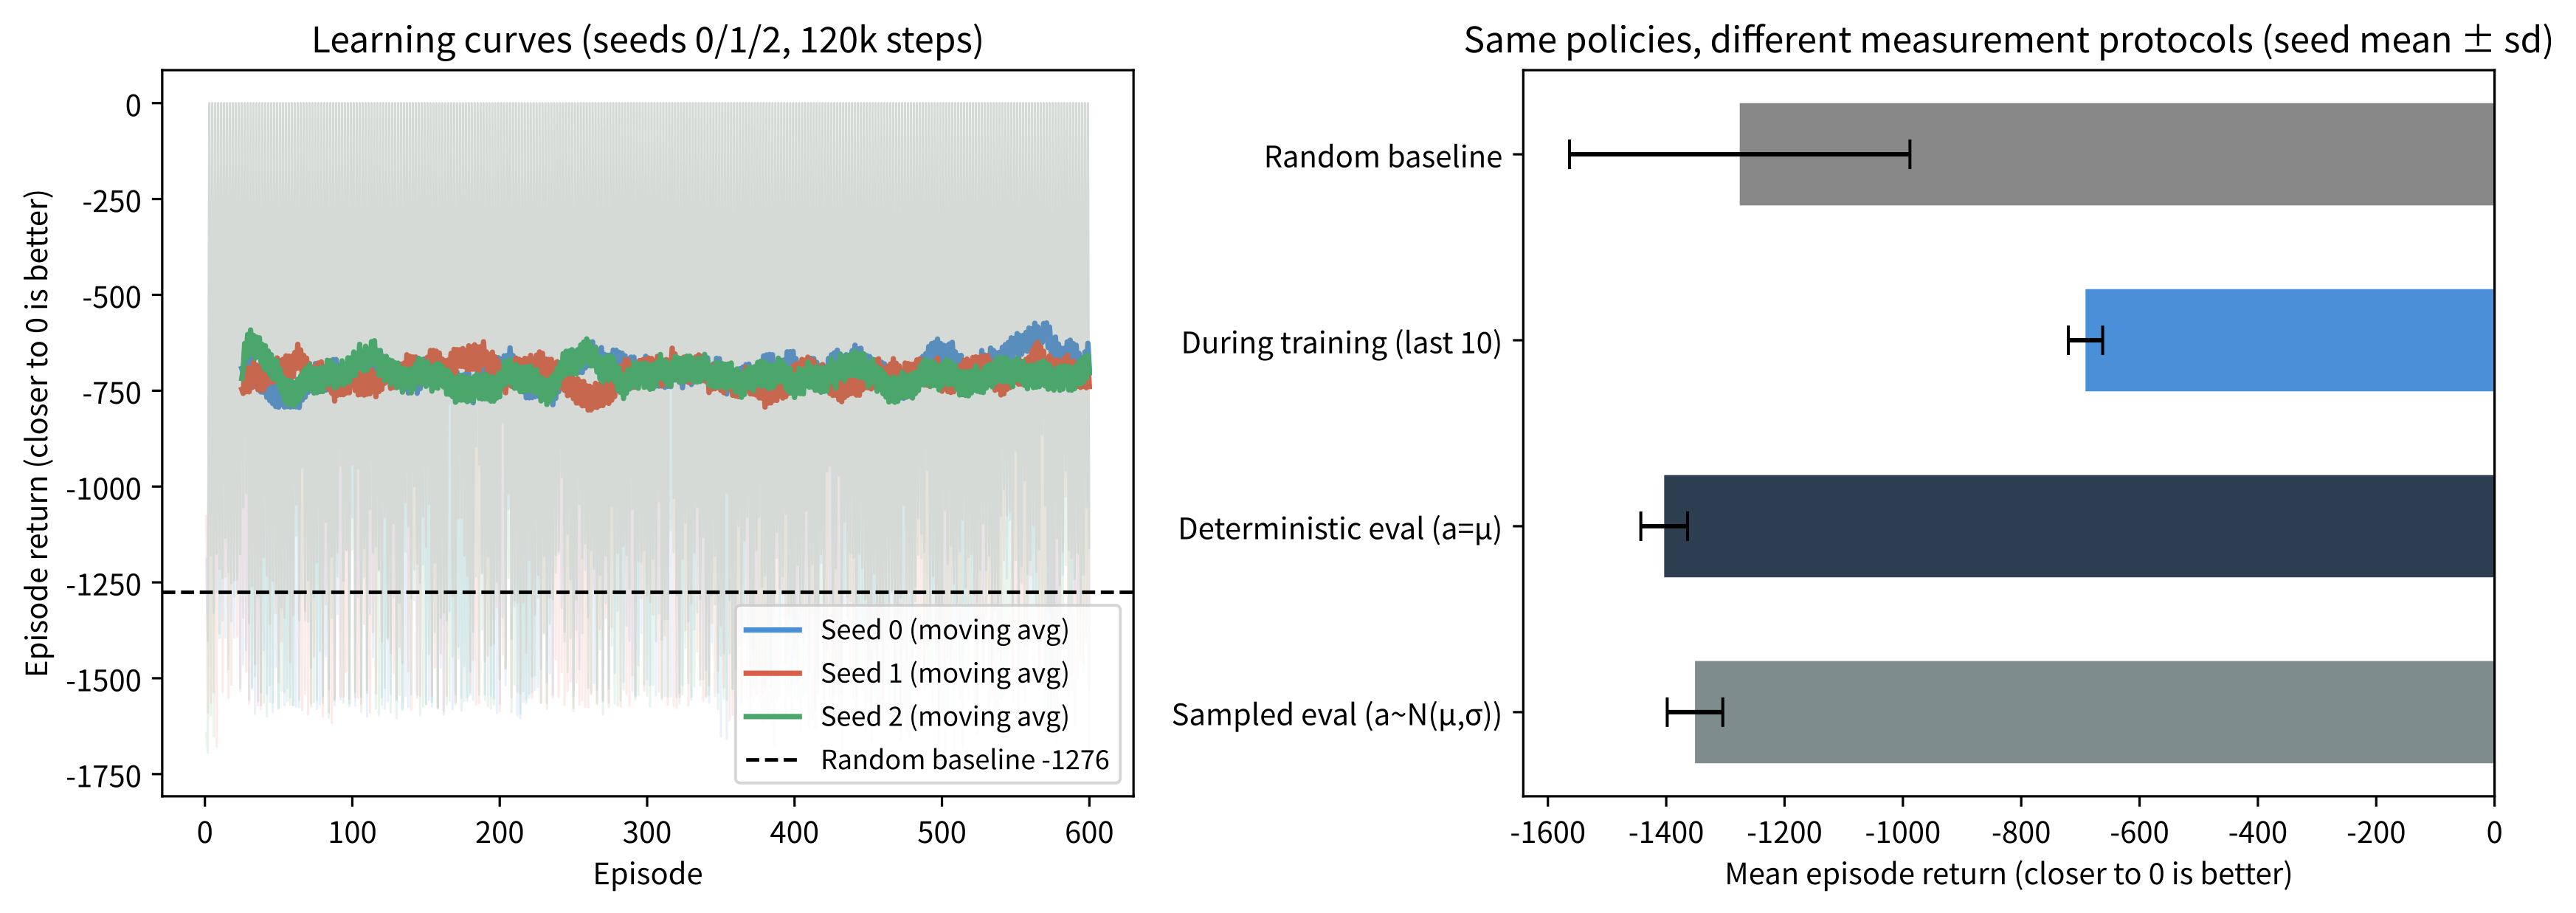
\includegraphics[width=\linewidth]{ch16_1_ppo_seed_curves.png}
      \vskip0.3em
      {\footnotesize 좌: 학습 곡선 (검정 점선 = 무작위 베이스라인 $-1274$,
      시드마다 모양이 다르면 정상). 우: 같은 세 정책을 \textbf{네 가지
      측정 방식}으로 — 학습 도중(탐험 포함)이 베이스라인을 크게 상회해도
      결정적 $a=\mu$는 그 아래일 수 있음.}
    \end{column}
  \end{columns}
\end{frame}

\begin{frame}{하이퍼파라미터 선택의 주의}
  \begin{itemize}
    \item ``학습 곡선이 예뻐질 때까지 $\gamma$/$\lambda$/$\epsilon_{\text{clip}}$을
      조한다'' — 지도학습에서 ``val 곡선이 예뻐질 때까지 조정''하는 것과
      같은 역할 (ML1 Ch6.2). 그 자체로 \textbf{정당한 모델 선택}.
    \item 단, 두 조건:
      \begin{enumerate}
        \item 어떤 곡선(학습 도중 리턴의 이동평균)을 보고 고르기로 정했는지를
          보고서에 \textbf{기록}할 것.
        \item 최종 \textbf{결정적} 평가는 선택된 파라미터로 \textbf{한 번만}
          돌려야 한다.
      \end{enumerate}
    \item ``결정적 평가가 예뻐질 때까지'' 조정하는 것은 \textbf{평가에 대한
      과적합} — ML1 6.2의 ``test는 한 번만'' 원칙이 그대로.
    \item 선택 기준의 \textbf{사전 기록}이 ``정당한 val 선택''과
      ``평가 과적합''의 구분선이다 (16.2 체크리스트 ``실험 프로토콜의
      정직성'' 항목에서 바로 감점 대상).
  \end{itemize}
\end{frame}

\begin{frame}{전체 그림: 4주 파이프라인}
  \begin{columns}[T]
    \begin{column}{0.5\textwidth}
      \begin{itemize}
        \item 8.1절 파이프라인과 \textbf{대칭} — \textbf{환경
          $\to$ 알고리즘·구현 $\to$ 평가·정당화 $\to$ 발표}.
        \item 각 박스가 Block B 어느 절의 원칙을 집행하는지 함께 적음.
        \item \textbf{붉은 점선}(평가 $\to$ 구현·실험)이 핵심: 시드 간 편차가
          비정상적으로 크거나 프로토콜 결함이 발견되면 \textbf{돌아가서
          다시} 돌려야 한다는 뜻.
        \item ``한 번 지나가면 돌아올 수 없는'' 것은 \textbf{최종 발표뿐} —
          그 외 모든 단계는 되돌아갈 수 있다.
      \end{itemize}
    \end{column}
    \begin{column}{0.48\textwidth}
      \centering
      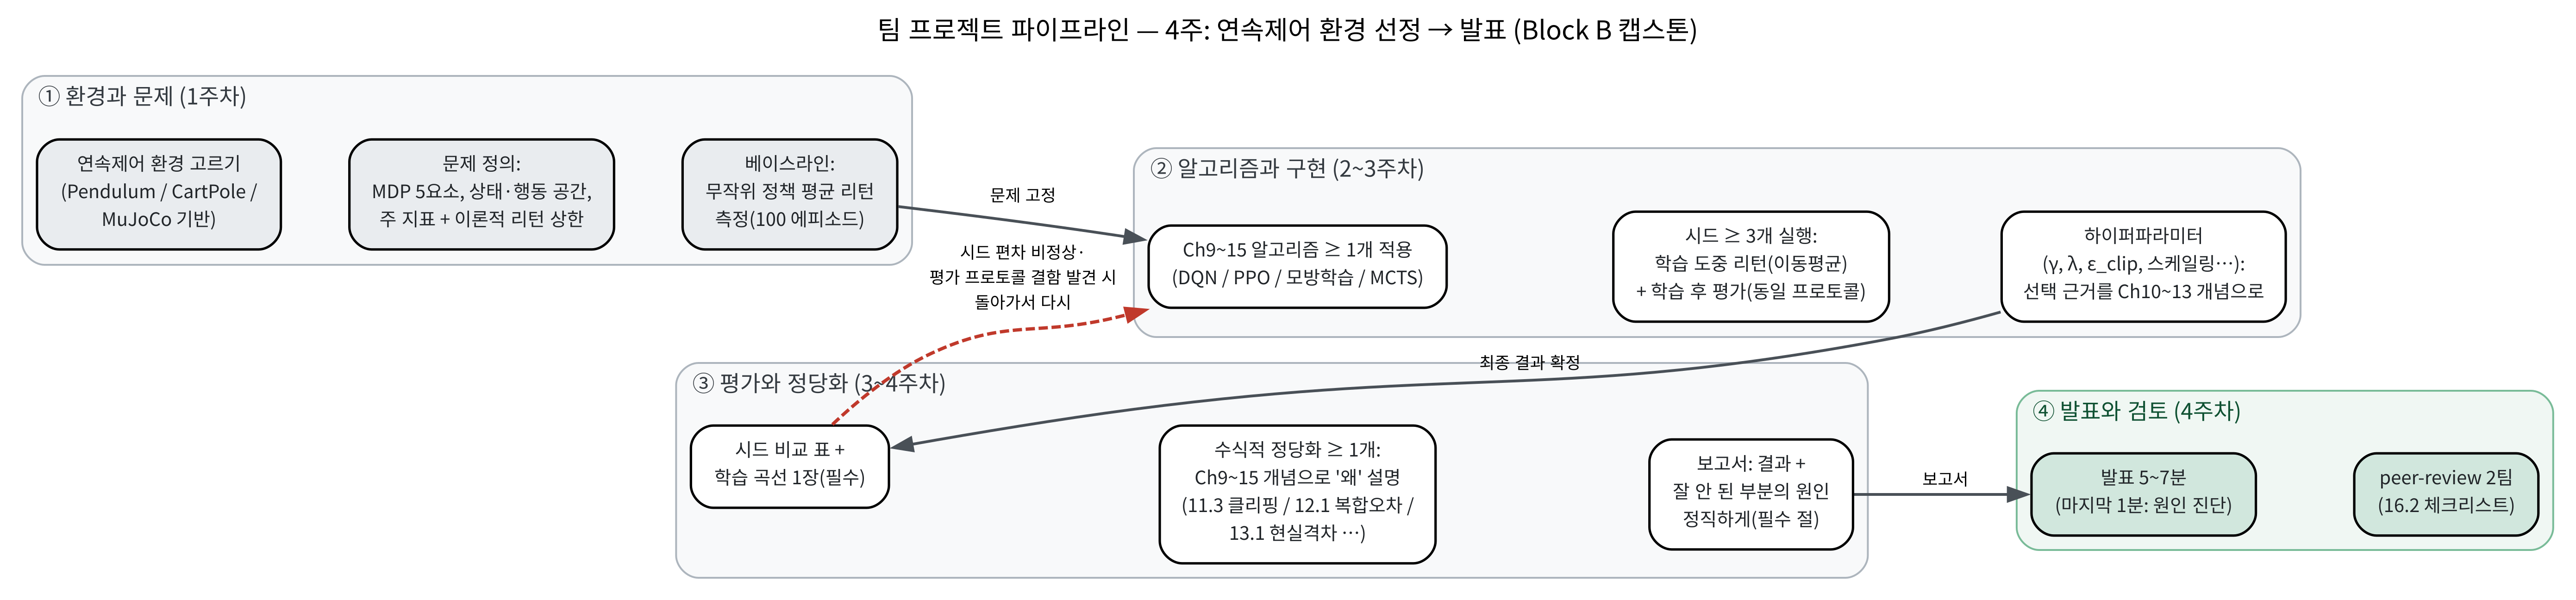
\includegraphics[width=\linewidth]{ch16_1_capstone_pipeline.png}
      \vskip0.3em
      {\footnotesize 1주: 환경 고르기·문제 정의·베이스라인 / 2$\sim$3주: 알고리즘
      구현·시드 $\geq 3$·하이퍼파라미터 / 3$\sim$4주: 시드 비교 표·학습
      곡선·보고서 / 4주: 발표·peer-review.}
    \end{column}
  \end{columns}
\end{frame}

\begin{frame}{일정과 마일스톤 — M1$\sim$M4가 제출물}
  \small
  \begin{tabular}{@{}p{0.52\textwidth}p@{}}
    \toprule
    \textbf{주 / 해야 할 일} & \textbf{마일스톤(제출)} \\
    \midrule
    \textbf{1}주: 환경 후보 2$\sim$3개 조사, \textbf{문제 정의 문서}(MDP
    5요소, 주 지표와 리턴의 이론적 범위), \textbf{베이스라인(무작위) 리턴
    측정} & \textbf{M1} 문제 정의 + 환경 선택 + 베이스라인 숫자 (1p) \\
    \textbf{2}주: Ch9$\sim$15 코드 재사용으로 알고리즘 $\geq$1개 구현,
    \textbf{시드 1개에서 엔드투엔드 동작 확인}(Pendulum 12만 스텝
    $\approx$20$\sim$30초), \textbf{학습 예산 추정} & \textbf{M2} 중간코드
    리뷰(코드 + 베이스라인 + e2e 숫자) \\
    \textbf{3}주: 나머지 시드 실행, 하이퍼파라미터 조정(모두 동일
    프로토콜), \textbf{학습 후 결정적 $a=\mu$ 평가}(시드마다 동일
    에피소드 수), 학습 곡선·시드 비교 표 도출 & \textbf{M3} 학습 곡선
    1장 + 시드 비교 표 \\
    \textbf{4}주: 수식적 정당화, 보고서·슬라이드 완성, \textbf{발표
    5$\sim$7분}, peer-review 2팀 & \textbf{M4} 보고서 + 발표 + 리뷰 2건 \\
    \bottomrule
  \end{tabular}
  \vskip0.8em
  \begin{block}{왜 M2에 ``학습 예산 추정''이 들어가는가}
    Block A(표 기반)에서는 1에피소드 1초라 예산이 문제가 안 됐지만, Block B
   에서는 Pendulum 12만 스텝이 CPU 22초인 반면 MuJoCo 대형과제의 100만 스텝은
    수 \textbf{시간} — \textbf{계산 전에 ``얼마나 걸리는가''를 계획하는 것
    자체가 방법론의 정직성}에 포함. (Pendulum 12만 스텝 $\approx$22초가
    ``정상 기준선''.)
  \end{block}
\end{frame}

\begin{frame}[fragile]{수식적 정당화: 좋은 예와 나쁜 예}
  \footnotesize
  \textbf{설정}: 어떤 팀이 Pendulum에 PPO를 적용해 ``학습이 잘
  됐다''고 발표. 11.2 스크래치패드로 실행 검증한 실제 결과:
\begin{lstlisting}
처음 10 에피소드 평균 리턴:  -1551.7
마지막 10 에피소드 평균 리턴: -1092.2
\end{lstlisting}
  {\color{ksared}\textbf{나쁜 설명}}: ``학습 곡선이 올라갔다. PPO가 잘
  작동했다.''
  \vskip0.3em
  {\color{ksagolddk}\textbf{좋은 설명}}: ``12만 스텝(300 iteration) 동안
  평균 리턴이 $-1551.7 \to -1092.2$로 약 30\% 개선 — \textbf{다만 완전히
  수렴한 수준은 아니고} 여전히 개선 여지. 이 개선은 보상을 1/8 스케일링하고
  $\gamma=0.95$, $\lambda=0.9$로 조정한 뒤에야 나타남 — Ch11.3의 GAE
  $\lambda$(편향-분산 트레이드오프)가 ``왜 그렇게 골랐는지''의 답.
  처음 시도(스케일링 없음, $\gamma=0.99$)는 오히려 나빠짐 — Ch11.1대로
  어드밴티드 추정의 \textbf{분산이 너무 커}서 클리핑이 그 노이즈를
  충분히 걸러내지 못했기 때문으로 추정.''
  \vskip0.5em
  {\footnotesize 두 설명은 같은 방향(개선됨)을 말하지만, 좋은 설명만
  (1) 정확한 수치, (2) ``완전 수렴 아님''의 정직함, (3) 하이퍼파라미터의
  이론적 근거를 담는다 — 이것이 ``수식적 정당화''의 실제 의미.}
\end{frame}

\begin{frame}{보고서 구조 (M4) — 발표 슬라이드 = 보고서의 절 제목}
  \small
  \begin{enumerate}
    \item \textbf{문제 정의} (0.5p): MDP 5요소(Ch3.1), 상태·행동 차원과
      범위, 전이·보상(이론적 리턴 범위 포함), 할인율, \textbf{주 지표}
      (학습 후 결정적 평가의 평균 리턴), \textbf{베이스라인}.
    \item \textbf{알고리즘 선택과 이유} (1p): \textbf{왜 이 환경을 이
      알고리즘에 골랐는가}(§페어링의 ``무대'' 논리), 하이퍼파라미터
      ($\gamma, \lambda, \epsilon_{\text{clip}}$, 보상 스케일)와 선택
      근거(Ch10$\sim$13 개념).
    \item \textbf{실험 프로토콜} (1p): 시드 목록, 학습 예산,
      \textbf{평가 프로토콜(결정적 $a=\mu$, 에피소드 수, 모든 시드에 동일)
      명시}, 하이퍼파라미터 선택 절차. \textbf{이 절이 없으면 16.2
      체크리스트에서 바로 감점.}
    \item \textbf{결과} (1p): 시드 비교 표, 학습 곡선 1장(여러 시드를
      얇은 선으로), \textbf{``같은 정책 여러 측정'' 패널}(학습
      도중/결정적/베이스라인).
    \item \textbf{수식적 정당화} (1p): Ch9$\sim$15 개념 $\geq 1$개로
      ``왜 이 결과가 나왔는지'' — ``좋은 예'' 문체로.
    \item \textbf{잘 안 된 부분과 원인 진단} (0.5p): \textbf{필수} —
      안 된 부분이 없었으면 ``무엇을 시도했다가 안 됐는가''를 쓴다.
      ``모두 잘 됐다''는 보고서는 이 절이 비어 있다는 뜻.
  \end{enumerate}
\end{frame}

\begin{frame}{채점 기준 (rubric)}
  \small
  \begin{tabular}{@{}llp{0.44\textwidth}@{}}
    \toprule
    항목 & 비중 & 좋은 답 \\
    \midrule
    문제 정의와 환경 & 15\% & MDP 5요소·차원·지표·베이스라인·리턴 이론
    범위가 명확, 환경 선택이 ``개념 X가 돋보이는 무대'' 논리로 근거됨 \\
    방법론 적절성 & 20\% & Ch9$\sim$15 알고리즘이 환경 특성(연속/이산,
    보상 희소성)에 맞았고, 하이퍼파라미터 근거가 배운 개념으로 설명됨 \\
    \textbf{실험 프로토콜의 정직성} & \textbf{25\%} & 시드 $\geq 3$,
    동일 평가 프로토콜(결정적, 동일 에피소드 수), 베이스라인, 예산과 선택
    절차가 보고서에서 추적 가능 \\
    수식적 정당화 & 20\% & 배운 개념 $\geq 1$개로 ``왜''를 설명했고,
    그 설명이 \textbf{실제로 관측한 숫자와 일치} \\
    \textbf{결과의 정직성과 반성} & \textbf{20\%} & 불안정했던 시드·구간,
    베이스라인 이하의 평가치를 숨기지 않고 Ch9$\sim$15 개념으로 진단 \\
    \bottomrule
  \end{tabular}
  \vskip0.8em
  \begin{block}{정직성 항목이 \textbf{합계 45\%}인 이유}
    이 프로젝트의 목적은 ``좋은 정책을 만든 것''이 아니라 \textbf{그 성능
    숫자를 정직하게 얻는 절차를 실제로 수행한 것}을 증명. 결정적 평가가
    베이스라인을 못 넘겨도 프로토콜이 정직하면 높은 점수, 반대로 숫자가
    예뻐도 \textbf{시드 1개였다면} ``프로토콜의 정직성''에서 크게 감점.
  \end{block}
\end{frame}

\begin{frame}{자주 하는 실수 5가지 — 16.2 리뷰의 ``반박 가능한 질문''이 된다}
  \small
  \begin{enumerate}
    \item \textbf{시드 1개 실험으로 결론} — 같은 PPO라도 시드만 바꿔도
      마지막 10 평균이 $\pm100\sim200$ 흔들림(실습표: $-668\sim-732$).
      알고리즘 간 차이가 시드 간 sd보다 작으면 결론은 ``유의미한 차이
      관측 불가''. \emph{리뷰 질문: ``시드 간 sd가 방법 간 차이보다 커요?''}
    \item \textbf{학습 도중 리턴을 ``최종 정책 성과''로 보고} — 학습 도중
      마지막 10($-673\sim-732$)은 $\sigma$ 샘플링 노이즈가 섞인 ``탐험
      포함 성과''. ``곡선이 올랐다''를 ``잘 학습됐다''로 번역하는 순간
      읽기 3의 격차(결정적 $-1403$ vs 베이스라인 $-1274$)가 사라진다.
    \item \textbf{결정적 평가가 예뻐질 때까지 하이퍼파라미터 조정} —
      학습 곡선으로 조정하는 것은 정당한 val 선택이지만, \textbf{최종
      평가치를 보며 조정하면 평가에 과적합}(ML1 6.2 ``test는 한 번만'').
      구분선 = 선택 기준의 \textbf{사전 기록}.
    \item \textbf{베이스라인 없이 ``잘 배웠다''} — 무작위 리턴($-1274$)을
      재지 않고 ``$-1400$, 꽤 좋다''라고 발표 = 그 숫자가 무작위보다
      \emph{나쁜}지도 모름. zero-torque($\approx-1230$)까지 함께 재면
      기준선 두 개가 생긴다.
    \item \textbf{``결정적 $\ll$ 샘플 평가는 버그''로 오해} — $a=\mu$가
      $a\sim\mathcal{N}$보다 낮은 것은 \textbf{정상}. 격차의 크기는
      ``정책이 탐험 운에 얼마나 의존하는가''의 측정값 — \textbf{작을수록}
      정책이 자기 $\mu$만으로 선다.
  \end{enumerate}
\end{frame}

\begin{frame}{발표 — 5$\sim$7분, 마지막 1분이 가장 평가받는다}
  \begin{itemize}
    \item 구성: 문제 정의(1분) $\to$ 알고리즘과 이유(2분) $\to$ 학습 곡선
      + 수식적 정당화(2$\sim$3분) $\to$ \textbf{잘 안 됐던 부분과 원인
      진단(1분)}.
    \item ``최종 결정적 리턴이 얼마였는가''보다 \textbf{``왜 이 알고리즘을
      이 환경에 골랐고, 왜 이 결과가 나왔는가''}에 더 높은 점수.
    \item 마지막 1분 = rubric의 \textbf{``결과의 정직성과 반성''} 항목이
      정확히 보는 곳.
  \end{itemize}
  \vskip0.5em
  {\footnotesize \textbf{예}(실습 숫자를 그대로 발표): ``PPO를 시드 3개로
  12만 스텝 학습. 학습 도중 마지막 10은 $-673/-732/-668$으로 무작위
  ($-1274$)보다 2배 정도 낫다. \textbf{다만} 학습 후 결정적($a=\mu$)
  평가는 $-1358/-1454/-1398$으로 베이스라인 \emph{아래}였다 — 11.2 FAQ의
  ``에피소드 리턴 자체의 분산은 줄일 수 없다''대로, 학습 도중 숫자에는
  $\sigma$ 샘플링의 운이 섞여 있었고, 노이즈를 빼면 12만 스텝으로는 $\mu$가
  아직 정확하지 않다는 진단. 13$\sim$14절의 수백만 스텝 원리로 \textbf{예산
  10배 실행}을 계획하고 있다.''}
  \vskip0.4em
  ``실패에 가까운 실험''까지 \textbf{배운 개념으로 해석한} 발표가 더 높은
  점수를 받는다 — ``모든 것이 잘 됐다''는 발표는 이 항목에서 \textbf{스스로
  감점}을 받는 것.
\end{frame}

\begin{frame}{실습: 캡스톤 프로토콜 6단계를 코드로}
  \small
  \begin{enumerate}
    \item \textbf{(M1) 문제 정의} — Pendulum-v1의 MDP: 관찰 3차원
      $[\cos\theta, \sin\theta, \dot\theta]$, 행동 1차원 토크 $[-2,+2]$ Nm,
      200스텝, 보상 $r=-\theta^2-0.1\dot\theta^2-0.001a^2$(상한 0).
    \item \textbf{베이스라인} — 무작위 정책 100 에피소드 ($-1274.1$,
      sd 300).
    \item \textbf{(M2) 구현} — Ch11.2의 \texttt{ActorCritic} + GAE 코드를
      \textbf{재사용}(8.1 FAQ ``코드를 처음부터 써야 하나요?''의 답과
      같은 이유).
    \item \textbf{(M3) 시드 0/1/2} — 같은 파라미터($\gamma=0.99$,
      $\lambda=0.95$, $\epsilon_{\text{clip}}=0.2$)로 12만 스텝씩
      (시드당 20$\sim$30초), 학습 도중 리턴 비교.
    \item \textbf{학습 후 평가} — 세 정책을 (a) 결정적 $a=\mu$,
      (b) 샘플 $a\sim\mathcal{N}(\mu,\sigma)$로 각각 50 에피소드 평가 후
      베이스라인과 비교.
    \item \textbf{발표 자료용 한 장} — 좌: 시드별 학습 곡선, 우: ``같은
      정책, 측정 방식 네 가지'' 막대.
  \end{enumerate}
  \vskip0.4em
  \begin{block}{이 6단계의 의미}
    곧 §보고서 구조의 6개 절, 다시 16.2절의 체크리스트로 매핑된다 —
    \textbf{같은 절차를 세 가지 언어(코드, 보고서, 리뷰)로 말할 수 있어야}
    이 프로젝트가 끝난 것이다.
  \end{block}
\end{frame}

\begin{frame}{확인 문제 (1)-(2)}
  \small
  \begin{itemize}
    \item \textbf{1.} 시드 0의 학습 도중 마지막 10이 $-673.5$(베이스라인
      $-1274$의 2배)인데, 결정적 평가는 $-1357.9$(베이스라인 \emph{아래})다.
      어느 쪽이 ``배운 정책의 진짜 성능''이고, \textbf{주 지표}는 무엇이어야
      하는가?
      \vskip0.2em
      {\footnotesize $\to$ \textbf{결정적($a=\mu$) 평가}가 탐험을 뺀
      본래 실력(8.1의 $\varepsilon=0$ greedy 평가에 해당). 학습 도중 리턴은
      ``탐험 포함 성과''. 주 지표는 \textbf{결정적 평가} — 평가의 목표가
      ``정책의 안정적인 성능''이지 ``학습 과정이 잘 봤는가''가 아니기
      때문. 학습 곡선은 ``학습이 실제로 되고 있었는가''의 증거로,
      \textbf{역할을 구분해 함께} 보고.}
    \item \textbf{2.} ``연속 정책에는 $\varepsilon$이 없으니, 평가할 때
      $\sigma$ 파라미터를 0으로 설정해서 돌리면 되지 않나요?'' — 왜
      오답인가?
      \vskip0.2em
      {\footnotesize $\to$ $\sigma$는 \textbf{학습된 파라미터}(엔트로피
      보너스와 함께 학습 대상) — $\sigma=0$로 바꾸면 ``원래 정책에서 탐험을
      제거한 실행''이 아니라 \textbf{파라미터를 바꾼 \emph{다른} 정책}의
      실행. 정답: 파라미터를 그대로 두고 \textbf{$a=\mu_\theta(s)$(평균)만
      내보내는 것} — ``같은 정책을 샘플링 없이 실행''하는 것이
      $\varepsilon=0$과 동일한 역할.}
  \end{itemize}
\end{frame}

\begin{frame}{확인 문제 (3)-(4) + 자주 묻는 질문}
  \small
  \begin{itemize}
    \item \textbf{3.} ``PPO 결정적 평가가 $-900$으로 30\% 개선됐다''는
      발표에 던질 \textbf{3점 질문 2개}: (a) \emph{프로토콜의 정직성}:
      ``시드를 몇 개로 확인했어요? 시드별 숫자는요?'' (b) \emph{결과의
      정직성}: ``결정적 평가는 몇 에피소드로 잤나요? 베이스라인은 몇
      에피소드로?'' — 50 에피소드 결정적 평가의 시드당 sd가 186$\sim$239로
      커서 평가 에피소드 수가 적으면 측정 오차와 구별 불가. (추가: ``학습
      예산(스텝 수)은 같았나요?'' — 12만 vs 100만 스텝 비교는 알고리즘이
      아니라 \textbf{예산} 비교.)
    \item \textbf{4.} 12만 스텝 $\approx$22초(1시드)일 때, 100만 스텝
      (8.3배)을 시드 3개로 돌리면 $\approx$\textbf{10분 내외}. \textbf{M2에서}
      해야 하는 이유: M3의 ``남은 시드 실행''이 \textbf{예산 계획 없이는
      시작할 수 없기} 때문 — Humanoid(수백배)에 적용하면 수 시간이 되고,
      그제서야 ``새벽에 돌리자/시드를 줄이자''의 결정. ``얼마나 걸리는가''
     는 실험 \textbf{설계의 일부}이지 행정 절차가 아니다.
  \end{itemize}
  \vskip0.4em
  {\footnotesize \textbf{FAQ} — 수렴하지 않았어도 발표하는가? \textbf{된다} —
  ``완전 수렴 아님''을 정직하게 보고하고 원인 진단하는 것이 부풀린 성공보다
  낫다. / 알고리즘 2개가 비슷한가? \textbf{비슷함 자체가 관찰} — 학습
  도중/학습 후를 나눠 비교하면 다른 트레이드오프가 드러남. / 시드 몇 개가
  정석인가? Pendulum은 1시드 20$\sim$30초라 \textbf{3$\sim$5개가 현실적
  하한}, MuJoCo 대형은 3개 + GPU 배분 고려. / PPO가 12만 스텝으로 베이스라인
  못 넘기면? \textbf{예외가 아니라 일반} — Pendulum은 완전 수렴에 100만
  스텝 이상. 성공 기준 = 정직한 절차 + 정당화. / 라이브러리
  (stable-baselines3)를 써도 되나? \textbf{된다} — 다만 ``그대로 쓴
  부분''(기본값)과 ``팀이 바꾼 부분''(환경 인터페이스, 예산, $\gamma/\lambda$,
  평가 프로토콜)을 \textbf{구분}해야 하고, (b)가 실질적 산출물.}
\end{frame}

\section{16.2 Peer-Review}

\begin{frame}{왜 이번 주가 ``역전''의 주인가}
  \begin{itemize}
    \item 16.1에서 각 팀은 \textbf{발표팀}으로서 자신의 프로젝트를 5$\sim$7분
      안에 설명했다. 이번 블록(16.2)에서는 역할이 역전된다 —
      \kb{이번에는 네가 심사위원이다}.
    \item 다른 두 팀의 발표를 듣고, 체크리스트를 적용해 \textbf{리뷰 두 통}을
      작성하고, 그 리뷰의 \emph{질}로 채점받는다.
    \item ``왜 반박 가능한 질문이 좋은 리뷰인가''의 근거(Popper의 반증주의,
      Amgen 재현 실험: 53편 중 6편만 재현 성공, 2011)는 ML1 8.2 / ML2 8.2에서
      다뤘다 — 여기서는 \textbf{신경망 강화학습이라는 새 대상에 무엇을
      추가하는가}만 다룬다.
  \end{itemize}
\end{frame}

\begin{frame}{심사 대상이 8.2에서 달라진 두 가지}
  \begin{columns}[T]
    \begin{column}{0.5\textwidth}
      \kb{첫째 — 알고리즘이 신경망에 올랐다}
      \begin{itemize}
        \item DQN(Ch09) · REINFORCE·Actor-Critic(Ch10) · PPO(Ch11) ·
          모방학습(Ch12) · 시뮬레이션(Ch13$\sim$14) · MCTS(Ch15).
        \item 8.2: ``CliffWalking에 SARSA vs Q-learning이 맞는가'' —
          \textbf{한 장의 개념}으로 판단 가능.
        \item 16.2: ``Pendulum(연속 행동)에 DQN을 쓴 팀'' — \textbf{왜} DQN이
          부적합한지(행동 공간의 \textbf{이산성 전제}, Ch09)까지 짚어야
          한다.
      \end{itemize}
    \end{column}
    \begin{column}{0.5\textwidth}
      \kb{둘째 — 시드 질문이 ``신경망 특유의 새 얼굴''로}
      \begin{itemize}
        \item (a) \textbf{초기화} 자체가 매번 다르다(무작위 가중치).
        \item (b) 학습이 \textbf{수만$\sim$수백만 스텝}이라 ``12만 스텝이면
          충분히 수렴했는가''를 판정하기 어렵다.
        \item (c) 하이퍼파라미터($\gamma, \lambda$, 클리핑 $\epsilon$, 보상
          스케일)가 결과에 \textbf{지대하게} 영향.
      \end{itemize}
      $\Rightarrow$ 같은 ``반박 가능한 질문''이 \textbf{수치 민감성} 질문으로
      번역된다: ``시드 2개를 더 돌리면 이동평균의 편차가?''(Ch11.2),
      ``보상을 1/8로 스케일링한 게 결과의 방향을 바꿨나요?''(Ch11.3).
    \end{column}
  \end{columns}
\end{frame}

\begin{frame}{이번 주는 어떻게 진행되는가}
  \small
  \begin{tabular}{@{}clp{0.4\textwidth}@{}}
    \toprule
    순서 & 내용 & 시간 배분 \\
    \midrule
    1 & 다른 두 팀의 발표 청취(팀당 5$\sim$7분, 16.1 형식) + 보고서·
      코드시트 열람 & 약 30분 \\
    2 & \textbf{작성 리뷰 2통} — 팀당 체크리스트 5항목 + 반박 가능한
      질문 $\geq 1$개(개념의 장·절 명시) & 발표 직후(각 10분) \\
    3 & 질의·토론 — 리뷰어가 쓴 질문에 발표팀이 그 자리에서 답변 &
      나머지 시간 \\
    \bottomrule
  \end{tabular}
  \vskip0.8em
  \begin{block}{핵심 = 2번의 \textbf{작성 리뷰}}
    3번 토론은 ``발표팀이 그 질문에 \emph{실제로} 답할 수 있는가''를 가르는
    자리 — \textbf{새로운 계산·실험}(시드 재실행, 평가 프로토콜 변경,
    베이스라인 실측, 하이퍼파라미터 민감성 실험)을 꺼내야 답하는 질문이
    \textbf{3점}이고, ``네, 알겠습니다''로 넘겨질 질문은 2점에 머문다.
    16.1에서 ``수식적 정당화''가 발표팀의 \emph{의무}였다면, 이번 주
    그 \emph{타당성}을 리뷰어가 \emph{심사}하는 것.
  \end{block}
\end{frame}

\begin{frame}{Peer-Review 체크리스트 — 5항목}
  \small
  \begin{tabular}{@{}ll@{}}
    \toprule
    항목 & 확인할 것 \\
    \midrule
    \kb{환경 설명} & 상태·행동·보상이 명확히 정의됐는가 \\
    \kb{알고리즘 선택} & 환경의 특성(이산/연속 행동, 보상의 희소성 등)에
    알고리즘이 맞았는가 \\
    \kb{수식적 정당화} & 요구사항을 충족했고, 실제로 관찰한 결과와
    일치하는가 \\
    \kb{결과의 정직성} & 수렴하지 않은 부분·학습이 불안정했던 구간을
    숨기지 않고 원인을 분석했는가 \\
    \kb{탐험-활용 균형} & Chapter 2에서 배운 딜레마가 실제 학습 곡선에서
    어떻게 드러났는가 \\
    \bottomrule
  \end{tabular}
  \vskip0.8em
  5항목은 16.1 채점 기준의 \textbf{축 그대로} — 리뷰어와 발표팀이
  \textbf{같은 기준표}를 공유해야 ``감점''과 ``좋은 지적''이 \textbf{같은
  언어}로 이야기될 수 있다.
\end{frame}

\begin{frame}{5항목의 구체적 의미 (1) 환경 설명 · (2) 알고리즘 선택}
  \small
  \begin{itemize}
    \item \kb{(1) 환경 설명} — MDP 5요소(Ch03.1) 중 \textbf{상태·행동·보상}이
      보고서에서 추적 가능한지. ``Pendulum을 썼다'' 한 줄만 있고 \emph{주
      지표가 무엇인지}(학습 도중 리턴? 이동평균? 평가 리턴?), \emph{리턴의
      부호 규약}(항상 음수, 0에 가까울수록 좋음)이 없으면 뒤의 모든
      숫자가 ``무엇의 평균''인지 모른다. 학습 곡선이 \emph{에피소드
      단위}인지 \emph{스텝 단위} 평균인지도 여기서.
    \item \kb{(2) 알고리즘 선택} — ``PPO를 골랐다''가 아니라,
      \textbf{이 환경의 어떤 특성}이 그 선택을 정당화하는지.
      \begin{itemize}
        \item \textbf{연속 vs 이산} 행동 공간이 \textbf{가장 먼저} 봐야
          하는 분기: DQN(Ch09)은 \emph{이산} 행동을 전제로 $Q(s,a)$를
          표처럼 출력 — 연속(Pendulum, Reacher)에 그대로 쓰면 ``행동을
          어떻게 이산화했는가''의 추가 전제가 붙는다.
        \item \textbf{희소} 보상(Ch15.2의 보너스 구조)도 근거: 희소 보상에
          DQN은 Q값의 \emph{희소성 문제}(대부분 스텝이 0이라 학습 신호
          약함)를 겪는다.
      \end{itemize}
  \end{itemize}
\end{frame}

\begin{frame}{5항목의 구체적 의미 (3)-(5) 정당화 · 정직성 · 탐험-활용}
  \small
  \begin{itemize}
    \item \kb{(3) 수식적 정당화} — ``최소 1개''를 채웠는지는 \emph{형식}
      문제, 이 항목은 \emph{내용}: 짚은 개념(예: Ch11.3 GAE $\lambda$)이
      \textbf{실제로 관찰한 숫자와 일치}하는가. ``$\lambda$가 편향-분산을
      조절한다''는 문장만 있고 $\lambda$를 바꿔 \emph{어드밴티지 분산이
      어떻게 변했는지} 실측이 없으면, 그 문장은 \emph{어디에나 붙을}
      설명일 뿐.
    \item \kb{(4) 결과의 정직성} — 신경망 \textbf{초기화 시드}를 몇 개
      돌렸는지, 시드별 이동평균이 \emph{사라지지 않고} 보고에 들어갔는지,
      ``완전 수렴 아님''을 숨기지 않는지. ``결과가 좋았는가''가 아니라
      ``결과가 \textbf{정직한 절차}로 얻어졌는가''를 본다.
    \item \kb{(5) 탐험-활용 균형} — Ch02 멀티암 밴딧의 딜레마가
      \textbf{실제 학습 곡선}에서 어떻게 드러나는지. 신경망 RL에서는
      탐험이 $\varepsilon$-greedy(DQN, Ch09.2)나 가우시안 정책의 $\sigma$
      (Ch10.2, Ch11.2)로 구현 — ``탐험을 줄여가는데 줄이는 시점이 학습
      곡선의 어떤 지점이었나? 일찍 줄이면 고착, 늦으면 노이즈''(Ch02
      직관의 신경망 버전 검증).
  \end{itemize}
\end{frame}

\begin{frame}{채점 기준: ``채웠는가''가 아니라 ``구체적인가''}
  \small
  \begin{tabular}{@{}llp{0.4\textwidth}@{}}
    \toprule
    리뷰 품질 & 특징 & 예시 (Pendulum PPO) \\
    \midrule
    \textbf{1점 — 감상평} & 구체적 지적 없음. 듣기만 하고 느낌만 적음 &
    ``학습 곡선이 완만하게 올라가서 PPO가 잘 작동한 것 같습니다.'' \\
    \textbf{2점 — 일반 지적} & 문제를 제기하지만 \emph{근거(개념)}가
    약함. 발표팀이 ``네''로 넘길 수 있음 & ``시드를 하나 더 돌려서
    확인해보는 게 좋을 것 같습니다.'' \\
    \textbf{3점 — 반박 가능한 질문} & 이 학기 개념(장·절)을 명시하고,
    \emph{답이 나쁘면 결과가 흔들리는} 질문 & ``시드 2개를 더 돌리면
    이동평균의 표준편차가 얼마나 되나요? 두 알고리즘 간 차이가 그 편차보다
    큰가요? 아니면 시드의 우연일 가능성이 있나요(Ch11.2)?'' \\
    \bottomrule
  \end{tabular}
  \vskip0.8em
  \begin{block}{1점 $\to$ 3점의 공통 패턴 (ML1 8.2와 똑같다)}
    추상적 평가어(``잘됐다'', ``확인해보라'')를
    \textbf{(a) 구체적 관찰 + (b) 이 학기 개념(Ch NN) + (c) 그것이 왜
    문제인지(숫자)}로 교체. ``시드를 하나 더 돌려라''(2점)에는 관찰도
    개념도 없지만, 3점 질문에는 \textbf{관찰(시드 수) + 개념(Ch11.2
    초기화 민감성) + 왜 문제인지(숫자 비교)}가 모두 들어 있다.
  \end{block}
\end{frame}

\begin{frame}{손으로 한 번: 가상 발표 (팀 ``진자돌림'')}
  {\footnotesize 실습 노트북과 동일한 설정 — 모든 숫자는 \emph{실제로
  그렇게 실행하면} 나오는 것. 문제인 곳은 숫자가 아니라
  \textbf{프로토콜}.}
  \vskip0.4em
  \begin{block}{발표 요약}
    ``Pendulum-v1에 PPO. 300 반복 $\times$ 400 스텝(총 12만 스텝),
    $\gamma=0.99$, $\lambda=0.95$, 클리핑 $\epsilon=0.2$, 보상 스케일링
    없음, \textbf{시드 42 하나}로 학습. 처음 10 에피소드 평균 리턴
    $-805.3 \to$ 마지막 10 에피소드 평균 $-742.0$으로 개선. 학습 곡선이
    완만하게 올라가서 PPO가 잘 작동했다. Chapter 11에서 배운 클리핑
    덕분에 안정적인 학습이 됐다.''
  \end{block}
  \vskip0.4em
  체크리스트 5항목을 하나씩 적용해 본다 — 문제는 모두 \textbf{숫자가
  아니라 보고의 구조}에 있다.
\end{frame}

\begin{frame}{가상 발표를 체크리스트로 — (1)(2) 환경 · 알고리즘}
  \small
  \begin{itemize}
    \item \textbf{환경 설명} — 환경 자체는 명확하다(Pendulum-v1, 연속
      행동 1차원 토크, 항상 음수 리턴). 그러나 \textbf{주 지표가
      모호하다} — ``마지막 10 에피소드 평균''이 \emph{학습 도중} 에피소드
      리턴인지, 학습 \emph{후}(탐험 없이) 재평가한 리턴인지 문장에
      없다. 8.1/16.1의 ``비교 프로토콜''이 둘을 \textbf{반드시
      나눠서} 보고하게 한 이유가 바로 이 모호함.
    \item \textbf{알고리즘 선택} — PPO는 연속 행동 환경(Pendulum)에
      맞는 선택(Ch10$\sim$11). \textbf{이 항목은 통과}.
  \end{itemize}
\end{frame}

\begin{frame}{가상 발표를 체크리스트로 — (3)(4)(5)}
  \small
  \begin{itemize}
    \item \textbf{수식적 정당화} — Ch11을 \emph{인용}했지만, 인용과
      관측이 \textbf{연결되어 있지 않다}. ``클리핑 덕분에 안정적''은
      \emph{어디에나 붙을} 설명 — 클리핑 $\epsilon$을 \emph{바꿔서}
      안정성(곡선 변동폭, 발산 여부)이 어떻게 변했는지 실측이 없으면,
      그 문장은 \emph{이 실험에 붙은} 정황이 아니라 \emph{책에서 읽은}
      문장일 뿐.
    \item \textbf{결과의 정직성} — 세 가지가 \textbf{사라져 있다}:
      (1) \textbf{시드 1개}(신경망 초기화가 무작위라 학습 과정의
      우연), (2) \textbf{베이스라인 부재}(무작위 정책 리턴 = ``잘
      배웠다''의 기준점), (3) \textbf{완전 수렴 여부 미명시}(12만
      스텝은 이 과제에 ``절반도 안'' 왔을 수 있음, 11.2).
    \item \textbf{탐험-활용 균형} — PPO의 탐험은 가우시안 $\sigma$(11.2)
     인데, $\sigma$가 학습 중 어떻게 변했는지(초기 $\approx 0.61$에서
      어디로) \textbf{한 마디도 없음} — Ch02 딜레마가 학습 곡선에
      어떻게 반영됐는지 확인 불가.
  \end{itemize}
\end{frame}

\begin{frame}{이 발표에 대한 3점 질문}
  \begin{block}{반박 가능한 질문}
    ``시드 42 하나로 ``마지막 10에피소드 평균 $-742.0$''이라고 했는데,
    \textbf{시드 2개를 더 돌리면} 그 평균의 \textbf{표준편차}가 얼마나
    되나요? 그리고 ``잘 배웠다''의 기준점인 \textbf{무작위 정책의 평균
    리턴}(약 $-1239$) 대비 얼마나 개선됐나요? 12만 스텝이면 11.2에서
    본 대로 ``절반도 안'' 온 수 있는데, 더 오래(예: 24만 스텝) 돌리면
    이동평균이 계속 올라가나요, 아니면 이미 \textbf{포화}인가요?''
  \end{block}
  \vskip0.5em
  \textbf{이 질문이 3점인 이유}: 발표팀이 답하려면 \textbf{새로운
  실험}(시드 2개 추가 + 무작위 베이스라인 실측 + 학습 스텝 확장)을
  돌려야만 하고, 그 실험을 돌리면 ``PPO가 잘 작동했다''는 결론이
  \textbf{흔들릴 수도} 있다 — 3점 조건(개념 명시 + 답이 나쁘면
  결과가 흔들림)을 정확히 만족.
\end{frame}

\begin{frame}{``우연히 좋은'' 패턴 5가지 — 신경망 RL 버전}
  {\footnotesize ML1 8.2의 ``우연히 좋은 결과'' 원천 = 테스트셋 유출·
  정확도의 함정·과적합. RL에는 \textbf{검증/테스트셋 자체가 없음} — 대신
  \textbf{학습 과정의 무작위성}이 같은 역할. 8.2의 5가지(표 기반)를
  \textbf{신경망} RL에 맞게 다시 쓴 것. 발표 슬라이드에서 이 패턴을
  보면 그 행의 ``반박 가능한 질문''을 바로 던져야 한다.}
  \vskip0.4em
  \small
  \begin{tabular}{@{}llp{0.46\textwidth}@{}}
    \toprule
    패턴 & 겉보기 & 실제로는 / 반박 가능한 질문 \\
    \midrule
    \textbf{1. 시드 1개 학습 곡선} & ``곡선이 완만하게 올라가네'' &
    신경망 \textbf{초기화}의 우연 — 같은 코드도 매번 다른 곡선.
    ``시드 2개를 더 돌리면 이동평균 sd가 얼마? 알고리즘 간 차이가
    그 편차보다 큰가요?''(Ch11.2 초기화 민감성) \\
    \textbf{2. 학습 도중 리턴으로 ``수렴'' 결론} & ``마지막 10이
    $-742.0$까지 올랐네'' & 학습 \emph{도중} 리턴은 탐험
    ($\sigma\cdot\varepsilon$ 포함)이 섞인 측정; 12만 스텝은 완전
    수렴이 아닐 수 있음. ``이 값은 학습 \emph{후} 탐험 0으로 재평가한
    값인가요? 더 오래 돌리면 포화인가요?''(11.2) \\
    \bottomrule
  \end{tabular}
\end{frame}

\begin{frame}{``우연히 좋은'' 패턴 3$\sim$5}
  \small
  \begin{tabular}{@{}llp{0.46\textwidth}@{}}
    \toprule
    패턴 & 겉보기 & 실제로는 / 반박 가능한 질문 \\
    \midrule
    \textbf{3. 하이퍼파라미터 ``적당히'' 하나} & ``$\gamma=0.99$,
    $\lambda=0.95$로 학습'' & 민감성 미검증 — Ch11.3 GAE $\lambda$
    (편향-분산)·$\gamma$(장기 리턴 비중)·\textbf{보상 1/8 스케일링}
    자체가 결과 방향을 바꿀 수 있음. ``$\lambda=0.8$이면 어드밴티지
    분산이? 스케일링이 결론의 방향을 바꿨나요?''(Ch11.3, 16.1 예시) \\
    \textbf{4. 이산용 알고리즘을 연속 환경에} & ``DQN으로 학습했다'' &
    DQN(Ch09)은 \emph{이산} 행동을 전제 — 연속 Pendulum에 쓰려면
    \emph{행동 이산화} 추가 전제가 \textbf{보고에 없으면} 선택 부적합.
    ``행동을 어떻게 이산화했나요? 정밀도 손실(Ch09) 확인했나요?
    연속 정책(Ch10$\sim$11)이 자연스러운데 왜 이산화?'' \\
    \textbf{5. 베이스라인 없이 ``잘 배웠다''} & ``$-742.0$가
    나왔다'' & 기준점 없이 ``나다''를 말할 수 없다 — Pendulum 무작위
    평균(약 $-1239$)을 \textbf{재야} 판정 가능. ``무작위 정책의 평균
    리턴은 얼마? 그 대비로 측정하셨나요?''(16.1 M2) \\
    \bottomrule
  \end{tabular}
  \vskip0.6em
  \textbf{패턴 3이 특히 신경망 \emph{특유}인 이유}: 8.2의 하이퍼파라미터
  ($\alpha, \varepsilon$)는 \emph{일치하는 스케일}에서 결과를 바꾸지만,
  신경망의 $\gamma\cdot\lambda\cdot$보상스케일은 \textbf{리턴의 규모
  ($-1000$ 안팎)를 직접 바꿔} ``좋아진 것''이 알고리즘의 공헌인지
  하이퍼파라미터의 공헌인지 \textbf{분리}하기 어렵다 — 16.1 ``좋은
  설명''이 ``보상 1/8 + $\gamma=0.95$ 조정 \emph{에야} 개선됐다''고
  \emph{명시}한 이유가 바로 이 분리.
\end{frame}

\begin{frame}{실습: 가상 발표를 \emph{리뷰어의 눈}으로 재실행}
  \small
  \begin{enumerate}
    \item \textbf{발표팀 재현} — Pendulum-v1, PPO(Ch11.2 코드), 시드 42,
      $\gamma=0.99$, $\lambda=0.95$, 300$\times$400(12만 스텝) $\to$
      처음 10: $-805.3$, 마지막 10: $-742.0$. 발표팀의 숫자 재현.
    \item \textbf{패턴 1 검증 — 시드 2개 추가} — 시드 123, 7로 재실행
      $\to$ 시드별 마지막 10 이동평균 표. 편차를 보고 ``알고리즘의
      차이''인가 ``시드의 우연''인가를 판정.
    \item \textbf{패턴 2 검증 — 학습 스텝 확장} — 12만 $\to$ 24만 스텝,
      이동평균이 포화되는지 $\to$ ``절반도 안 왔다''(11.2)를 숫자로
      확인.
    \item \textbf{패턴 3 검증 — 보상 스케일링 민감성} — 1/8 스케일링 +
      $\gamma=0.95$로 재실행 $\to$ 스케일링이 \emph{결론의 방향}을
      바꾸는지.
    \item \textbf{패턴 5 검증 — 베이스라인 실측} — 무작위 정책
      300 에피소드 $\to$ 평균 약 $-1239$.
    \item \textbf{리뷰 작성} — 실습에서 나온 숫자를 근거로 3점 리뷰를
      실제 템플릿(나중)으로 완성.
  \end{enumerate}
  \vskip0.4em
  {\footnotesize 이 6단계 = ``리뷰어는 발표팀의 실험을 \textbf{자기
  손으로} 재실행할 수 있는 사람''이라는 이 절의 핵심 태도를 코드
  레벨에서 보여줌. ``이 학습 곡선, 시드를 바꿔도 같은 모양이 나올까요?''
  라는 질문은 \textbf{리뷰어가 실제로 다시 돌려본 적}이 있을 때 가장
  날카롭다.}
\end{frame}

\begin{frame}{실제로 확인해본 것 — 같은 정책, 다른 프로토콜}
  \small
  \begin{itemize}
    \item 발표팀의 ``마지막 10 평균 $-742.0$''은 \textbf{학습 도중}
      에피소드 리턴의 이동평균. 같은 학습 결과를 \textbf{학습 후}에
      재평가하면: 탐험($\sigma\approx 0.61$)이 섞인 채 20 에피소드
      $\to$ \textbf{$-1413$}, 탐험 0(결정론적 $\mu$만) $\to$
      \textbf{$-1491$}. $-742.0$은 둘 다보다 \emph{훨씬} 좋아
      보인다.
    \item \textbf{왜?} 학습 도중 에피소드는 학습 \emph{초반}의
      에피소드(탐험이 크고 운 좋게 수직 근처를 스치는 것 포함)까지
      10개 평균에 들어가는 반면, 재평가는 \emph{마지막} 시점의 정책을
      순수하게 재기 때문. \textbf{같은 정책을 다른 프로토콜로 잰 값
      ($-742$ vs $-1413/-1491$)}이 8.2 패턴 2(평가 $\varepsilon$)의
      \textbf{신경망 버전} — $\varepsilon$ 대신 \emph{가우시안
      $\sigma$}가 탐험의 차원이 됐다.
    \item \textbf{베이스라인}까지: 무작위 300 에피소드 평균
      \textbf{약 $-1239$} — 발표팀 정책의 순수 재평가
      ($-1413/-1491$)는 \textbf{무작위보다 오히려 나쁘다}(12만 스텝의
      PPO가 아직 무작위 수준, 11.2 ``절반도 안 왔다''가 숫자로 확인).
    \item \textbf{시드}: 42/123/7의 마지막 10 평균 \textbf{$-742/-658/-568$}
      — 시드 간 sd(약 \textbf{70})가 주장한 ``개선폭''($-805\to-742$, 약
      63)보다 \textbf{크다}. ``개선됐다''의 \textbf{방향성조차} 시드의
      우연과 구별 불가 — 이 숫자들이 3점 질문이 \emph{왜} 3점인지를
      보여준다(답하려면 실제 실험을 돌려야 하고, 돌리면 결론이
      ``아직 무작위 수준''으로 \emph{뒤집힌다}).
  \end{itemize}
\end{frame}

\begin{frame}{리뷰 쓰는 과정 — 체크리스트 $\to$ 반박 가능한 질문}
  \begin{columns}[T]
    \begin{column}{0.5\textwidth}
      \begin{itemize}
        \item (1) 다른 팀 발표 + 보고서 읽고 \textbf{주장 파악}
          (알고리즘·하이퍼파라미터·숫자·결론)
        \item (2) \textbf{체크리스트 5항목} 적용
        \item (3) 각 항목에서 \textbf{질문 초안} — 답이 \emph{새
          계산·실험}이어야 함
        \item (4) \textbf{분기}: ``Ch9$\sim$15 개념(장·절)을 근거로
          들고, 답하려면 \textbf{새 실험}(시드 재실행·평가 프로토콜
          변경·베이스라인 실측·스케일 비교)이 필요한가?''
          \begin{itemize}
            \item 예 $\to$ \textbf{반박 가능한 질문 채택}(초록)
            \item 아니오 $\to$ ``곡선이 올라가네요'' 같은 \textbf{감상평}
              (빨강)으로 떨어짐 — Ch09.2($\varepsilon$-greedy)·Ch11.3
              (GAE $\lambda$)·Ch12.1(복합 오차) 개념으로 \textbf{다시
              쓰기}(점선으로 (3) 회귀)
          \end{itemize}
        \item (5) 3단계 기준(1/2/3점)으로 \textbf{자기 채점}
      \end{itemize}
    \end{column}
    \begin{column}{0.47\textwidth}
      \centering
      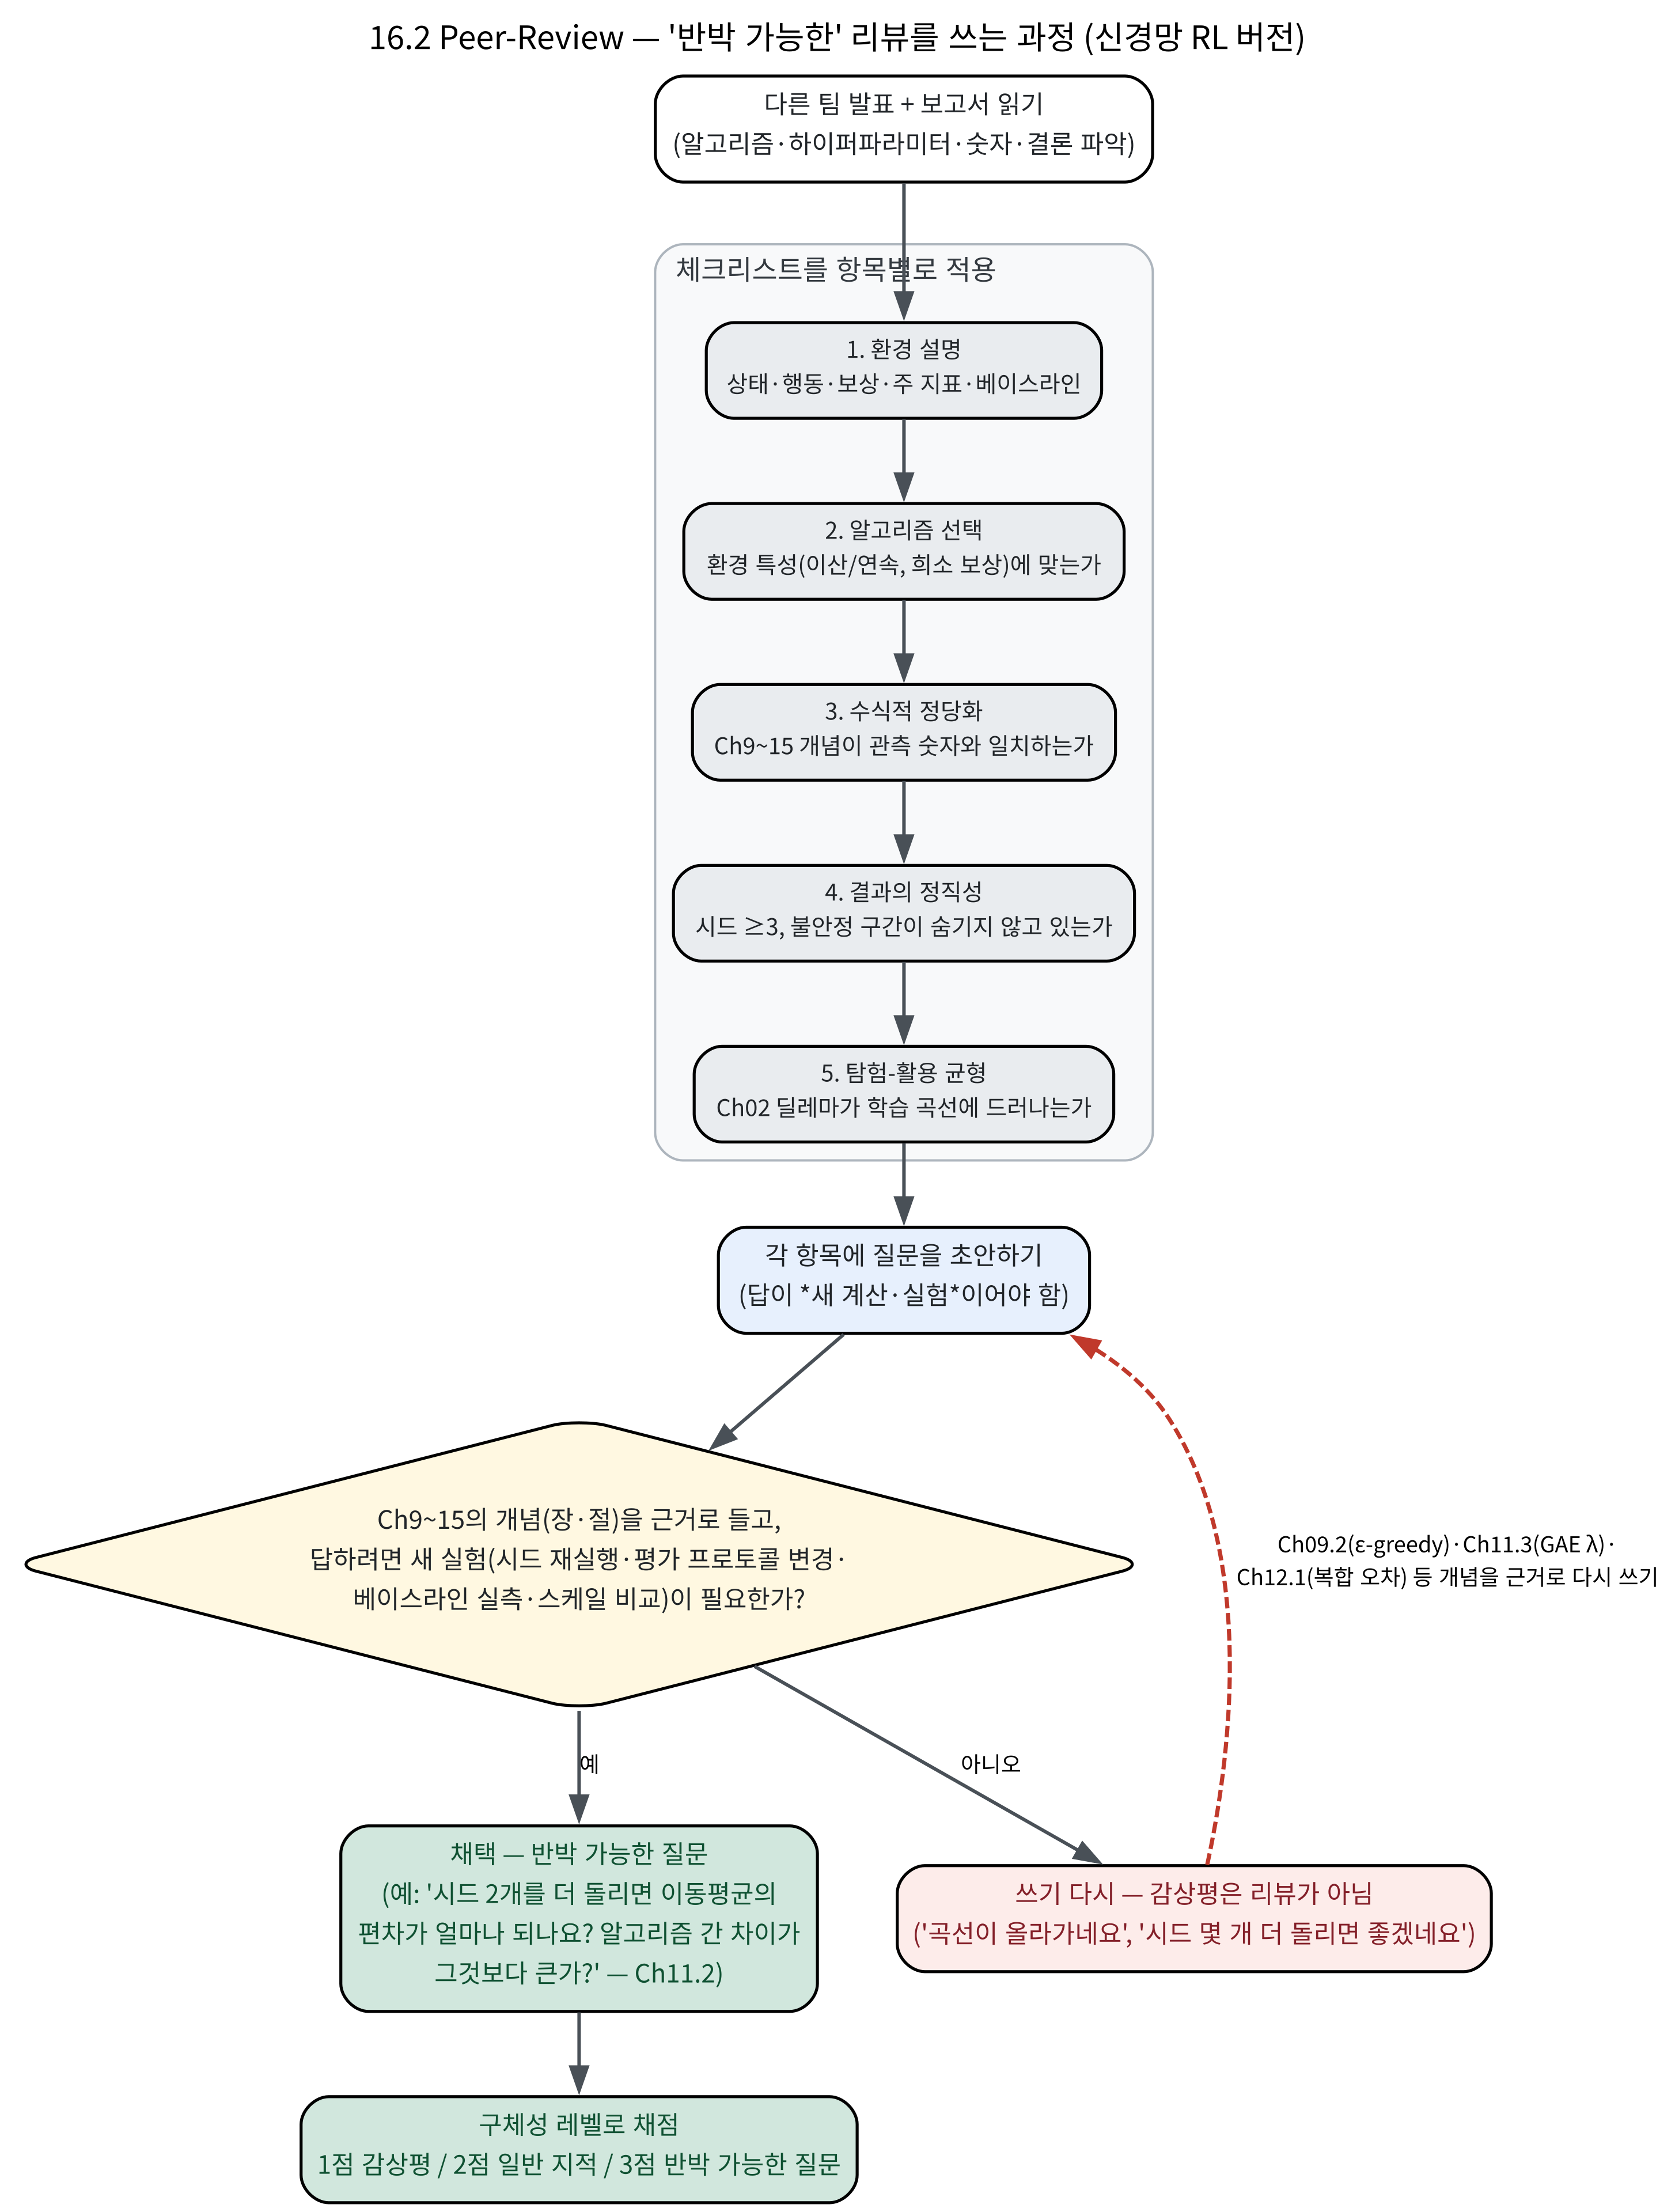
\includegraphics[width=\linewidth]{ch16_2_review_flow.png}
      \vskip0.3em
      {\footnotesize 신경망 RL 버전의 리뷰 플로우.}
    \end{column}
  \end{columns}
\end{frame}

\begin{frame}[fragile]{리뷰 템플릿 — ML1 8.2에서 5번을 두 칸으로}
  {\footnotesize ML1 8.2 템플릿에서 \textbf{5번을 두 칸으로 늘린 것}
  (``근거가 되는 개념'' + ``반박하려면 어떤 새 실험이 필요한지'')이
  강화학습 버전의 특징 — \textbf{답이 새 실험이어야} 질문이 3점이 되기
  때문. 5번 두 칸이 모두 채워져야 3점 도달; 비어 있으면
  \emph{반박 불가능}한 리뷰.}
\vskip0.3em
\begin{lstlisting}
팀 이름: ________   리뷰어: ________
1. 환경 설명 — 상태·행동(이산/연속)·보상(부호 규약, 희소 여부)·
   주 지표(학습중 리턴? 이동평균? 평가 리턴?)가 추적 가능한가?
   베이스라인(무작위) 리턴은 명시됐는가?
2. 알고리즘 선택 — 이 환경의 어떤 특성(행동 이산/연속, 보상 구조)이
   이 알고리즘(Ch9~15) 선택을 정당화하는가? 개념으로 설명되는가?
3. 수식적 정당화 — "≥1개"(16.1)를 채웠는가? 짚은 개념이
   실제로 관측한 숫자와 일치하는가(단순 인용이 아닌가)?
4. 결과의 정직성 — 시드(초기화) 수, 시드별 이동평균, "완전 수렴이
   아니다"가 정직하게 보고됐는가? 불안정한 시드·구간이 있는가?
5. 반박 가능한 질문 (필수, 1개 이상) —
   근거가 되는 개념: Chapter __ 절 __ (개념: ________)
   발표팀이 답하려면 필요한 새 실험/계산: __________________
   질문: ____________________________
   (발표팀이 이 질문에 답이 나쁘면 결과가 흔들리는 것이어야 한다)
\end{lstlisting}
\end{frame}

\begin{frame}{자주 하는 실수: 학습 곡선 한 번만 보고 결론 내리기}
  \small
  \begin{itemize}
    \item RL 프로젝트에서 특히 빈번한 부실한 리뷰: ``학습 곡선이 잘
      올라갔으니 성공''로만 판단 — 그 곡선이 \textbf{무작위 시드 하나}인지,
      \textbf{반복해서 일관된 경향}인지, \textbf{완전 수렴}인지
      ``개선됐지만 갈 길이 남은'' 상태인지를 \textbf{먼저} 물어야 한다.
    \item 신경망 RL에서 \emph{구조적으로} 더 위험한 이유: 곡선의
      ``오르다/안 오르다''가 \textbf{학습의 진전과 분리될 수 있기}
      때문 — 11.2에서 PPO 곡선은 ``완만한 상승''이었으나 개별
      에피소드 리턴은 $-1800$(쓰러짐) $\sim 0$(수직)까지 넓게
      퍼져 있음. 이동평균이 올라간다고 \textbf{에피소드 리턴의 분산}
      이 줄어든 것은 아니다.
  \end{itemize}
  \vskip0.4em
  \begin{block}{학습 곡선 3문 — 리뷰어가 던지는 질문}
    \begin{enumerate}
      \item \textbf{시드(초기화)}: 시드 \emph{몇 개}의 평균(또는 범위)
        인가? 1개라면 ``일관된 경향''을 말할 수 없다.
      \item \textbf{평가 프로토콜}: ``학습 도중 리턴''(탐험 포함)인지
        ``학습 후 탐험 0 재평가 리턴''인지? \textbf{다른 대상}의
        측정값이다.
      \item \textbf{수렴 여부}: 이 스텝 수(예: 12만)가 완전
        수렴인가? 더 오래 돌리면 포화인가요, 계속 오르나요(11.2)?
    \end{enumerate}
  \end{block}
\end{frame}

\begin{frame}{우리 팀 발표를 리뷰하기 — 발표 전 셀프-리뷰}
  \begin{itemize}
    \item ML1 8.2의 결론을 그대로: \kb{네가 심사할 때 던질 수 있는
      가장 날카로운 질문을, 네 발표 \emph{전에} 스스로 던져보고 답을
      준비해두는 것}이 최선의 전략.
    \item §5가지 패턴의 5개 질문을 \textbf{자기 팀의 보고서}에 적용:
      \begin{enumerate}
        \item 시드 3개의 이동평균 표가 \textbf{보고서에} 있는가
        \item 평가 프로토콜 문장(탐험 0? 에피소드 수? 모든 시드에 동일)이
          있는가
        \item 무작위 정책의 리턴이 \textbf{실측 숫자}로 적혀 있는가
        \item $\lambda\cdot$보상스케일 민감성을 \emph{한 줄이라도}
          검증했는가
        \item 불안정한 시드·구간이 ``잘 안 된 부분'' 절에 \emph{사라지지
          않고} 있는가
      \end{enumerate}
    \item 이 5가지에 답이 없다면, \textbf{발표 전에} 해결해두는 것이
      발표 중에 3점 리뷰를 받는 것보다 \textbf{항상 낫다}.
  \end{itemize}
\end{frame}

\begin{frame}{확인 문제 (1)-(2)}
  \small
  \begin{itemize}
    \item \textbf{1.} ``시드 3개 이동평균 $-742/-658/-568$이 나왔으므로
      PPO는 안정적이다'' — 이 세 숫자는 \textbf{무엇의} 편차이고,
      \textbf{무엇의} 편차가 \emph{아니}인가?
      \vskip0.2em
      {\footnotesize $\to$ \textbf{학습 과정의} 무작위성(초기화 시드)이
      만든 \textbf{세 개의 서로 다른 정책}의 이동평균 — ``어떤 정책이
      학습됐는가''의 편차이지 ``그 정책을 재는 측정 오차''가 아님.
      윈도우를 키워도 시드 간 편차(sd $\approx 70$)는 안 사라짐.
      ``안정적이다''라 말하려면 \textbf{두 층의 불확실성}을 구분해서
      (``시드 간 $\pm 70$, 시드 내 에피소드 분산 $\pm\ldots$'') 나눠
      적어야. 참고: 시드 간 편차(약 70)는 한 시드의 개선폭(약 63)보다
      크므로 방향성조차 우연과 구별 불가.}
    \item \textbf{2.} ``학습된 정책으로 마지막 10 에피소드 평균 $-742$''
      에는 어떤 \textbf{모순}이 숨어 있는가?
      \vskip0.2em
      {\footnotesize $\to$ ``학습된 정책''이 $\sigma$가 포함된 정책이라면
      ``마지막 10 에피소드''는 \textbf{탐험이 섞인} 측정 — PPO는 $\sigma$
      가 학습 중 변하므로(11.2), ``마지막'' 에피소드의 $\sigma$가 얼마
      였는지 명시해야 ``정책의 성과''. 질문: ``$\sigma$는 얼마?
      $\sigma=0$(결정론적)으로 재평가하면? 더 오래(30만 스텝) 하면
      포화되나요(11.2)?''}
  \end{itemize}
\end{frame}

\begin{frame}{확인 문제 (3)-(5)}
  \small
  \begin{itemize}
    \item \textbf{3.} ``GAE의 $\lambda=0.95$가 편향-분산을 조절해서
      학습이 안정됐다(Ch11.3)''로 끝난 정당화는 \textbf{2점에
      가깝다} — 개념은 인용했지만 \emph{관측 숫자가 없음}. 3점
      전환: ``$\lambda$를 0.8/1.0으로 바꿔 어드밴티지 \emph{추정치의
      분산}을 실측했습니다 — 실측 표가 보고에 있습니까?''(관찰+개념+
      숫자).
    \item \textbf{4.} ``왜 DQN이 아니라 PPO인가요?'' — 이대로면
      \textbf{2점}(``연속이라서'' 한 줄이면 반박이 어려움). 3점
      버전: ``Pendulum의 행동은 \emph{연속}인데 DQN(Ch09)은 \emph{이산}
      전제로 $Q(s,a)$를 출력 — 이산화의 \emph{정밀도 손실}을 확인했나요?
      아니면 연속 정책인 PPO(Ch10$\sim$11)가 자연스러운 이유가
      무엇인가요?''(체크리스트 2번에 Ch09 vs Ch10 개념 연결).
    \item \textbf{5.} ``PPO가 \emph{항상} 좋은가요? ``잘 학습했다''가
      무작위(약 $-1239$)보다 나은 걸 어떻게 아나요?'' — \textbf{정직한
      범위}: ``이 환경·이 설정($\gamma, \lambda$, 12만 스텝)에서 시드 3개
      한도에서 \emph{학습 도중} 이동평균이 무작위보다 높다''(단, 순수
      재평가 $-1413/-1491$로는 오히려 \emph{나쁨}; 외부 일반화는 이
      실험이 지지하지 않음). \textbf{말하면 안 될} 추론: ``PPO가 더 좋은
      알고리즘이다'' — 이 비교는 \emph{이 환경·이 스텝 수}의 답이지
      \textbf{알고리즘 우열}의 답이 아니다.
  \end{itemize}
\end{frame}

\begin{frame}{자주 묻는 질문}
  \small
  \begin{itemize}
    \item \textbf{하이퍼파라미터 선택 근거까지 물어봐야 하나?}
      \textbf{그렇다} — ``적당히'' 고른 값($\gamma, \lambda$,
      $\epsilon$, 보상 스케일)이 결과에 얼마나 큰 영향을 주는지 확인
      했는지가 \textbf{방법론 적절성} 평가의 핵심.
    \item \textbf{모방학습/MCTS 팀은 체크리스트를 어떻게?} ``학습
      곡선'' 대신 다른 증거로 — 모방학습: Ch12.1 \textbf{복합
      오차}(전문가 분포 밖 성능 저하) 관찰됐는가 / MCTS: Ch15.2처럼
      \textbf{시뮬레이션 횟수 증가} 시 선택되는 수가 더 정확해지는가.
    \item \textbf{문제가 없는 팀에 3점 질문을 어디서?} ``문제가
      \emph{보이지 않는} 것''과 ``\emph{확인되지 않은} 것''은 다르다 —
      3점 질문은 항상 \textbf{확인되지 않은 영역}에서 나옴(시드 5개
      확장, $\lambda$ 민감성, 더 긴 학습 스텝, 다른 평가 프로토콜).
      ``이 실험의 다음 단계로 무엇이 가장 정보가 많을까요?''가 3점이
      될 수 있다 — 발표팀이 답할 수 있다면 발표는 \textbf{더 단단해}
      짐(리뷰어가 목표 달성).
    \item \textbf{``더 오래 돌려보세요''를 쉽게 요구할 수 없는데?}
      리뷰어가 직접 300만 스텝을 돌릴 필요는 \textbf{없다} — 3점
      질문은 \emph{발표팀}이 돌려야 할 실험을 \emph{지적}하는 것.
      ``12만 스텝으로 포화가 안 보이는데, 이 과제는 완전 수렴에 수십만
      스텝이 필요하다고(11.2) 했죠? 그걸 \emph{인지하고} ``아직
      안 끝났다''고 보고했나요?'' — ``몰랐습니다''면 \textbf{수렴
      여부 미인식} 자체가 ``결과의 정직성'' 감점 요인.
  \end{itemize}
\end{frame}

\section{16.3 ML2 총정리와 학기를 넘어서}

\begin{frame}{이 절은 새로운 개념이 하나도 없다 — 하는 일 네 가지}
  \begin{enumerate}
    \item 16.1 발표 · 16.2 Peer-Review가 수렴해 온 \kb{채점 기준(rubric)}
      을 확정.
    \item \kb{같은 작은 MDP를 네 가지 경로로 풀어} ``모두가 같은
      방정식을 푸는 구조''를 \textbf{숫자}로 확인.
    \item 준비도를 스스로 재는 \kb{자가진단}(20문항).
    \item 학기 이후로 이어지는 지도(§학기를 넘어서)를 그림.
  \end{enumerate}
  \vskip0.6em
  \begin{block}{복습의 원칙}
    이 절의 모든 문장은 \textbf{이번 학기 13개 장의 요약} — 한 문장이라도
    막히면 \textbf{그 장·절 번호로 돌아가는 것}이 복습이 아니라
    \emph{정확한} 복습이다.
  \end{block}
\end{frame}

\begin{frame}{프로젝트 채점 기준 — Block B 3주가 수렴하는 곳}
  \small
  {\footnotesize 8.1 rubric이 그대로 이어져 오면서 ``Ch4$\sim$7 개념''이
  ``Ch9$\sim$15 개념''으로 교체된 것이 전부:}
  \vskip0.4em
  \begin{tabular}{@{}llp{0.42\textwidth}@{}}
    \toprule
    항목 & 비중 & 좋은 답이란 \\
    \midrule
    문제 정의와 환경 & 15\% & 상태·행동·보상이 명확(물리적 단위까지,
    Ch13), 환경 선택이 Ch9$\sim$15의 개념 검증 목적에 근거 \\
    알고리즘 적절성 & 20\% & 환경 특성(이산/연속, 희소성, 모델 유무)에
    알고리즘이 맞고, 근거가 Ch9$\sim$15 개념으로 설명 \\
    \textbf{실험 프로토콜의 정직성} & \textbf{25\%} & 시드 $\geq 3$,
    학습 곡선과 최종 평가(탐험 끔) 분리, 베이스라인(무작위 또는 사람이
    설계한 PD 제어 등), $\varepsilon\cdot\gamma\cdot\lambda\cdot$클립
    $\epsilon$ 감수성 실험이 보고서에서 추적 가능 \\
    수식적 정당화 & 20\% & 배운 개념 $\geq 1$개로 ``왜''를 설명(11.3
    클리핑, 12.1 복합 오차, 13.1 도메인 무작위화 $\ldots$)했고,
    관측 숫자와 일치 \\
    \textbf{결과의 정직성과 반성} & \textbf{20\%} & 불안정했던 시드·구간
    을 숨기지 않고 원인을 Ch9$\sim$15 개념으로 진단(16.1 좋은/나쁜 예
    기준) \\
    \bottomrule
  \end{tabular}
  \vskip0.5em
  \textbf{정직성 항목 = 합계 45\%} — 목적은 ``좋은 정책''이 아니라
  ``그 \textbf{성능 숫자를 정직하게 얻는 절차}를 실제로 수행했음을
  증명''. greedy 평가 $-1100$이 나와도 프로토콜이 정직하면 높은 점수,
  ``수렴했다''고 주장해도 시드 1개였다면 크게 감점 — 8.1의 ``\textbf{한
  번의 실행은 아무것도 말해주지 않는다}''가 연속 제어·신경망 무대에서
  다시 쓰인 것. 16.2의 5항목이 이 표의 열 \emph{그대로}인 이유도
  여기: \textbf{리뷰어와 채점자는 같은 눈으로 본 것}.
\end{frame}

\begin{frame}{손으로 한 번: Peer-Review rubric을 직접 써보기}
  \small
  \begin{itemize}
    \item 관점을 한 단계 더 뒤집어 \textbf{``너가 채점자라면 무엇을
      봐야 하는지'' rubric을 직접 쓰는 연습}.
    \item 5개 항목을 그대로 두고, 각 항목에 대해 \textbf{두 칸}을 채운다:
      (1) \textbf{나쁠 때는 어떤 모습인가}(구체적 나쁜 패턴), (2)
      \textbf{그걸 시험하는 질문은 무엇인가}(16.2의 반박 가능한 질문).
  \end{itemize}
  \vskip0.4em
  \begin{tabular}{@{}p{0.52\textwidth}p@{}}
    \toprule
    \textbf{나쁠 때 (구체적 패턴)} & \textbf{시험하는 질문 (반박 가능)} \\
    \midrule
    보고서에 \textbf{최고 점수 시드 하나만} 실려 있음. 학습 곡선이
    매끄럽고 불안정 구간 설명이 없는데, 학습 로그(코드 출력)를 보면
    300 iteration 중 \textbf{150$\sim$200 구간에서 리턴이 갑자기
    내려간} 기록이 있음 & ``로그의 150$\sim$200 iteration 리턴 추락을
    보고서의 학습 곡선에서 \textbf{왜 볼 수 없나요?} 그 구간을 자르면
    곡선이 매끄럽혀지나요?'' — \textbf{실제로 다시 돌려봐야} 답할 수
    있는 질문 \\
    \bottomrule
  \end{tabular}
  \vskip0.6em
  {\footnotesize 이 연습의 채점 기준 = 16.2 ``구체적인가'' 3단계
  그대로: ``나쁨 = 불성실''은 \textbf{1점}(감상평), 그날 발표실에서
  \emph{실제로 낚일 수 있는 패턴}을 쓴 것은 \textbf{3점}.
  ``나쁠 때의 모습''을 쓸 수 있으려면 ``좋은 답이란''을 이미 정확히
  이해해야 하므로, 이 30분 연습(나머지 4행 = 팀 회의 과제)은
  \textbf{학기 전체를 가장 빨리 재검증하는 방법}.}
\end{frame}

\begin{frame}{``달리거나 쉬거나'' MDP — 숫자로 보는 학기 중간고사}
  {\footnotesize 같은 작은 MDP를 Chapter 4$\sim$6의 네 경로로 풀어, 네
  경로가 ``같은 답, 또는 설명 가능한 다른 답''에 도달하는 것을 확인.
  실습 노트북이 네 경로의 학습 곡선을 코드로 재현.}
  \vskip0.4em
  MDP(8.3 템플릿 ②): 3-state, $\gamma = 0.9$
  \begin{itemize}
    \item \textbf{S}(시작): \emph{run} — 0.7 확률로 G, 0.3 확률로 S로
      \textbf{미끄러짐}, 보상 0. \emph{rest} — S에 남음, 보상 $-1$.
    \item \textbf{G}(골): \emph{collect} — T로 전이, 보상 $+3$.
    \item \textbf{T}: 터미널.
  \end{itemize}
  \vskip0.4em
  \begin{block}{경로 ① — 동적계획법(Ch4): 벨만방정식을 손으로 푼다}
    +3을 받는 유일한 길은 G에서 collect $\Rightarrow$ $V^*(G) = 3$.
    S에서 run이 최선(후보 추측)이면:
    \[V^*(S) = 0.9\big(0.7 \times 3 + 0.3\,V^*(S)\big)
      = 1.89 + 0.27\,V^*(S)
    \;\Longrightarrow\; V^*(S) = \frac{1.89}{0.73} \approx 2.589\]
    검증(후보+검증 Step 3):
    \[Q^*(S,\text{run}) = 2.589 \;>\;
    Q^*(S,\text{rest}) = -1 + 0.9 \times 2.589 = 1.330 \;\checkmark\]
  \end{block}
\end{frame}

\begin{frame}{경로 ② 몬테카를로(Ch5) · 경로 ③ SARSA(Ch6 on-policy)}
  \small
  \begin{itemize}
    \item \kb{경로 ② 몬테카를로} — greedy 정책(run@S, collect@G)으로
      에피소드를 끝까지 roll-out하고, 실제 리턴 $G_t$를 그대로 목표값으로
      (첫방문 MC). 4000 에피소드로 $V(S) \approx 2.594$ — 참값과
      \textbf{0.2\% 차이}. MC는 \textbf{편향이 없다}(실제 실현된 리턴의
      기댓값이 정확히 $V^\pi$) — ``충분히 많이 돌리면'' 약속이 이
      예에선 정말로 지켜진다.
    \item \kb{경로 ③ SARSA} — TD 오차로 갱신하되, 다음 행동 $a'$도
      \textbf{실제 행동 정책($\varepsilon$-greedy)}이 고른 것을 쓴다.
      \vskip0.2em
      \begin{block}{이번 학기의 핵심 드라마}
        \textbf{SARSA는 최적값이 아니라 ``탐험하는 행동 정책의 값''을
        배운다.} $\varepsilon=0.3$ 고정 시 $\pi$의 값 $V^\pi(S)
        \approx 2.29$로 수렴 — 해석적으로 \textbf{정확히 2.292}.
        \textbf{2.589가 아니라 2.29.}
      \end{block}
      (참고: 이때 $Q(S,\text{run})$ 자체는 $\approx 2.53$ — $\pi$가
      15\% 확률로 rest를 실제로 고르기 때문에
      $V^\pi(S) = 0.85\,Q^\pi(S,\text{run}) + 0.15\,Q^\pi(S,\text{rest})$
      가 \emph{실제 선택 분포}까지 반영해 더 낮아짐.)
  \end{itemize}
\end{frame}

\begin{frame}{경로 ③ SARSA — 0.297의 간극은 버그가 아니라 \emph{기능}}
  \small
  \begin{itemize}
    \item \textbf{2.589 $-$ 2.292 = 0.297}의 간극은 \textbf{버그가
      아니라 \emph{기능}} — ``$\varepsilon$-greedy가 30\%의 시간을
      미끄러지며 낭비한다''는 사실이 가치에 반영된 것 (6.3 CliffWalking
      에서 ``학습 도중 리턴이 오히려 나쁜'' SARSA의 근원이 바로
      여기).
    \item $\varepsilon$을 \textbf{감쇠}시키면(매 에피소드 0.995배
      스케줄) $V^\pi$는 $V^*$에 가까워진다 — $\varepsilon \to 0$이면
      행동정책이 greedy로 수렴하므로, 실습에서 \textbf{ε 감쇠 SARSA는
      2.589로 끝난다}.
  \end{itemize}
  \vskip0.5em
  {\footnotesize on/off-policy의 차이는 \textbf{취향이 아니라
  ``무엇을 묻느냐''}의 차이 — ③은 ``지금 탐험하는 정책의 값'',
  ④는 ``최적 값''. (확인 문제 3의 ``왜 PPO는 데이터를 재사용할 수
  없는가''의 표 버전이다.)}
\end{frame}

\begin{frame}{경로 ④ Q-learning(Ch6 off-policy) — $\max$ 한 줄}
  \small
  \begin{itemize}
    \item 갱신식에 \textbf{$\max$}을 써서, 행동 정책이 \emph{실제로
      무엇을 했든} ``다음에서는 \textbf{최선을 고른다면}''을 목표값으로
      삼는다.
    \item 그래서 행동 정책과 무관하게 \textbf{최적 $Q$에 직접 수렴} —
      시뮬레이션(2000 에피소드, $\varepsilon$을 0.05까지 감쇠) 결과
      $Q(S,\text{run}) \approx 2.64$, $Q(S,\text{rest}) \approx 1.34$,
      $Q(G,\text{collect}) = 3.0$ — 참값(2.589, 1.330, 3.0)에
      근접.
  \end{itemize}
  \vskip0.4em
  \small
  \begin{tabular}{@{}lllll@{}}
    \toprule
    경로 & 장 & 무엇을 쓰는지 & $V(S)$ 추정/수렴값 & 수렴 대상 \\
    \midrule
    ① 동적계획법 (손계산) & Ch4 & 전이 모델 $P$ & 2.589 & 최적값
    $V^*$ (정확) \\
    ② 몬테카를로 & Ch5 & 에피소드 전체 리턴 & 2.594 (4000 에피소드) &
    greedy 정책의 값 (편향 없음, 분산 큼) \\
    ③ SARSA & Ch6 & 1스텝 TD 오차 (on-policy) & \textbf{2.29}
    ($\varepsilon=0.3$ 고정) & \textbf{행동 정책} $\pi$의 값 $V^\pi$ \\
    ④ Q-learning & Ch6 & 1스텝 TD 오차 (off-policy) & 2.64
    (2000 에피소드, $Q(S,\text{run})$) & 최적값 $Q^*$ (근사) \\
    \bottomrule
  \end{tabular}
  \vskip0.6em
  ③과 ④의 갱신식은 \textbf{한 줄 차이}다 — 6.3에서 ``SARSA vs
  Q-learning의 차이는 $\max$ 한 줄''이라 했지만, 그 한 줄이
  \textbf{수렴하는 대상 자체를 바꾼다}:
\end{frame}

\begin{frame}[fragile]{한 줄 차이 — SARSA vs Q-learning}
\begin{lstlisting}
# SARSA (on-policy): 다음 행동 a_next는 ε-greedy가 실제로 고른 것
Q[s, a] += alpha * (r + gamma * Q[ns, a_next] - Q[s, a])
# Q-learning (off-policy): 실제로 무엇을 했든 "최선"을 목표로
Q[s, a] += alpha * (r + gamma * np.max(Q[ns])   - Q[s, a])
\end{lstlisting}
  \vskip0.6em
  \begin{block}{왜 1개 MDP를 \emph{네 번} 푸는가가 가치 있는가}
    단일 장에서는 보이지 않는 \textbf{세 가지}가 숫자로 드러난다.
    \textbf{(1) 목표가 다르면 답이 다르다} — ③④는 갱신식이 한 줄
    ($Q[ns,a']$ vs $\max Q[ns]$) 다른 구조인데 $V(S)$가 2.29와
    2.589에 각각 수렴 — 간극이 정확히 $V^* - V^\pi = 0.297$,
    ``탐험의 가격'' 그 자체. \textbf{(2) 네 경로 모두 같은
    방정식을 쓴다} — ①이 벨만방정식을 직접 풀고, ②는 미래 항을
    \emph{실제 실현}으로, ③④는 \emph{한 스텝 예측 + 자기 추정}으로
    대체한 것뿐. \textbf{(3) 탐험의 비용이 측정된다} — ③의 0.297
    간극은 ``$\varepsilon=0.3$의 탐험이 리턴 기준으로 이만큼
    값어치가 한다''는 \textbf{숫자} — Ch2에서 직관으로 시작한
    탐험-활용 딜레마가 여기서는 \emph{측정 대상}.
  \end{block}
\end{frame}

\begin{frame}{ML2 개념 지도 — 13개 장}
  \small
  \begin{tabular}{@{}llp{0.5\textwidth}@{}}
    \toprule
    장 & 배운 것 & 핵심 질문 \\
    \midrule
    Ch02 & 멀티암 밴딧 & 상태 없이도 탐험-활용 딜레마를 어떻게
    다루는가 \\
    Ch03 & MDP & 강화학습 문제를 어떻게 수학적으로 정식화하는가 \\
    Ch04 & 동적계획법 & 모델을 알 때 최적 정책을 어떻게 계산하는가 \\
    Ch05 & 몬테카를로 & 모델 없이, 에피소드 결과만으로 어떻게 배우는가 \\
    Ch06 & 시간차 학습 & 에피소드가 끝나길 기다리지 않고 어떻게
    배우는가 \\
    Ch07 & n-step/적격흔적/Dyna & MC와 TD 사이, 경험 재사용은 어떻게
    하는가 \\
    Ch09 & DQN & 표 대신 신경망으로 어떻게 Q-함수를 근사하는가 \\
    Ch10 & 정책기반 RL & Q를 거치지 않고 정책을 직접, 연속공간에서
    어떻게 학습하는가 \\
    Ch11 & PPO & 정책이 한 번에 너무 멀리 움직이지 않게 어떻게
    제한하는가 \\
    Ch12 & 모방학습/RLHF & 시행착오 대신 시연이나 선호로부터 어떻게
    배우는가 \\
    Ch13 & 로봇 시뮬레이션 & 물리 법칙이 지배하는 연속 제어 문제를
    어떻게 다루는가 \\
    Ch14 & MuJoCo/Isaac Sim & 시뮬레이션의 정밀도와 속도를 어떻게
    절충하는가 \\
    Ch15 & MCTS & 완벽한 모델이 있을 때 미리 수를 어떻게
    읽어보는가 \\
    \bottomrule
  \end{tabular}
\end{frame}

\begin{frame}{두 과목을 관통하는 구조 — 3단계}
  \begin{enumerate}
    \item \kb{모델을 정의한다}: 상태를 행동(또는 그 확률분포)으로
      매핑하는 함수의 형태를 정한다 (Q-테이블, 신경망 Q-함수, 정책
      신경망, 게임 트리, $\ldots$).
    \item \kb{틀린 정도(또는 목표와의 격차)를 수치화한다}: TD 오차,
      정책 그래디언트의 목적함수, PPO의 클리핑된 목적함수, MCTS의
      승률 통계, $\ldots$ — \textbf{형태는 매번 다르지만} ``지금이
      얼마나 좋은가/나쁜가를 수치 하나로 요약한다''는 \textbf{역할은
      항상 같}다.
    \item \kb{그 수치를 개선하는 방향으로 파라미터(또는 탐색 방향)를
      조정한다}: 경사하강법, 또는 트리 탐색의 반복 — \textbf{이
      학기 배운 모든 알고리즘의 마지막 단계는 결국 이것}.
  \end{enumerate}
  \vskip0.5em
  \begin{block}{``네 경로'' 예가 3단계의 축소판}
    앞의 4경로 예는 이 3단계가 \emph{같은 방정식} 위에서 어떻게
    변주되는지, 이 지도는 그 변주들이 어떤 축을 따라 정렬되는지를
    그려준다.
  \end{block}
\end{frame}

\begin{frame}{Block B 개념 지도 읽는 법 — 박스와 축의 교차점}
  \begin{columns}[T]
    \begin{column}{0.53\textwidth}
      지도의 읽기는 8.3 Block A 지도와 같은 \textbf{두 기법}:
      \begin{itemize}
        \item \kb{(1) 질문은 박스가 아니라 박스와 축의 \emph{교차점}} —
          ``DQN의 리플레이 버퍼가 왜 PPO에는 없는가'' = DQN 박스와
          on/off-policy 축이 만나는 \textbf{엣지}; ``GAE의 $\lambda$를
          0.95로 올리면 어떻게 되나'' = PPO 박스와 편향-분산 축의
          엣지.
        \item \kb{(2) 엣지가 곧 ``왜''} — 박스 자체를 묻는 질문은
          드물다. 발표·면접에서 반복적으로 나오는 것은:
          \begin{itemize}
            \item \textbf{신경망으로 바꾼 이유}(Ch9, 표가 불가능해진
              상태공간)
            \item \textbf{클립을 하는 이유}(Ch11, 한 번의 업데이트가
              정책을 망가뜨리는 방어)
            \item \textbf{모방학습이 나빠지는 이유}(Ch12, 분포 이동의
              복합 오차)
            \item \textbf{sim-to-real이 필요한 이유}(Ch13, 현실 격차가
              \emph{편이}이기 때문)
          \end{itemize}
        \item \textbf{이 4개 엣지를 각각 한 문장}으로 말할 수 있으면,
          지도는 끝난 것이다.
      \end{itemize}
    \end{column}
    \begin{column}{0.45\textwidth}
      \centering
      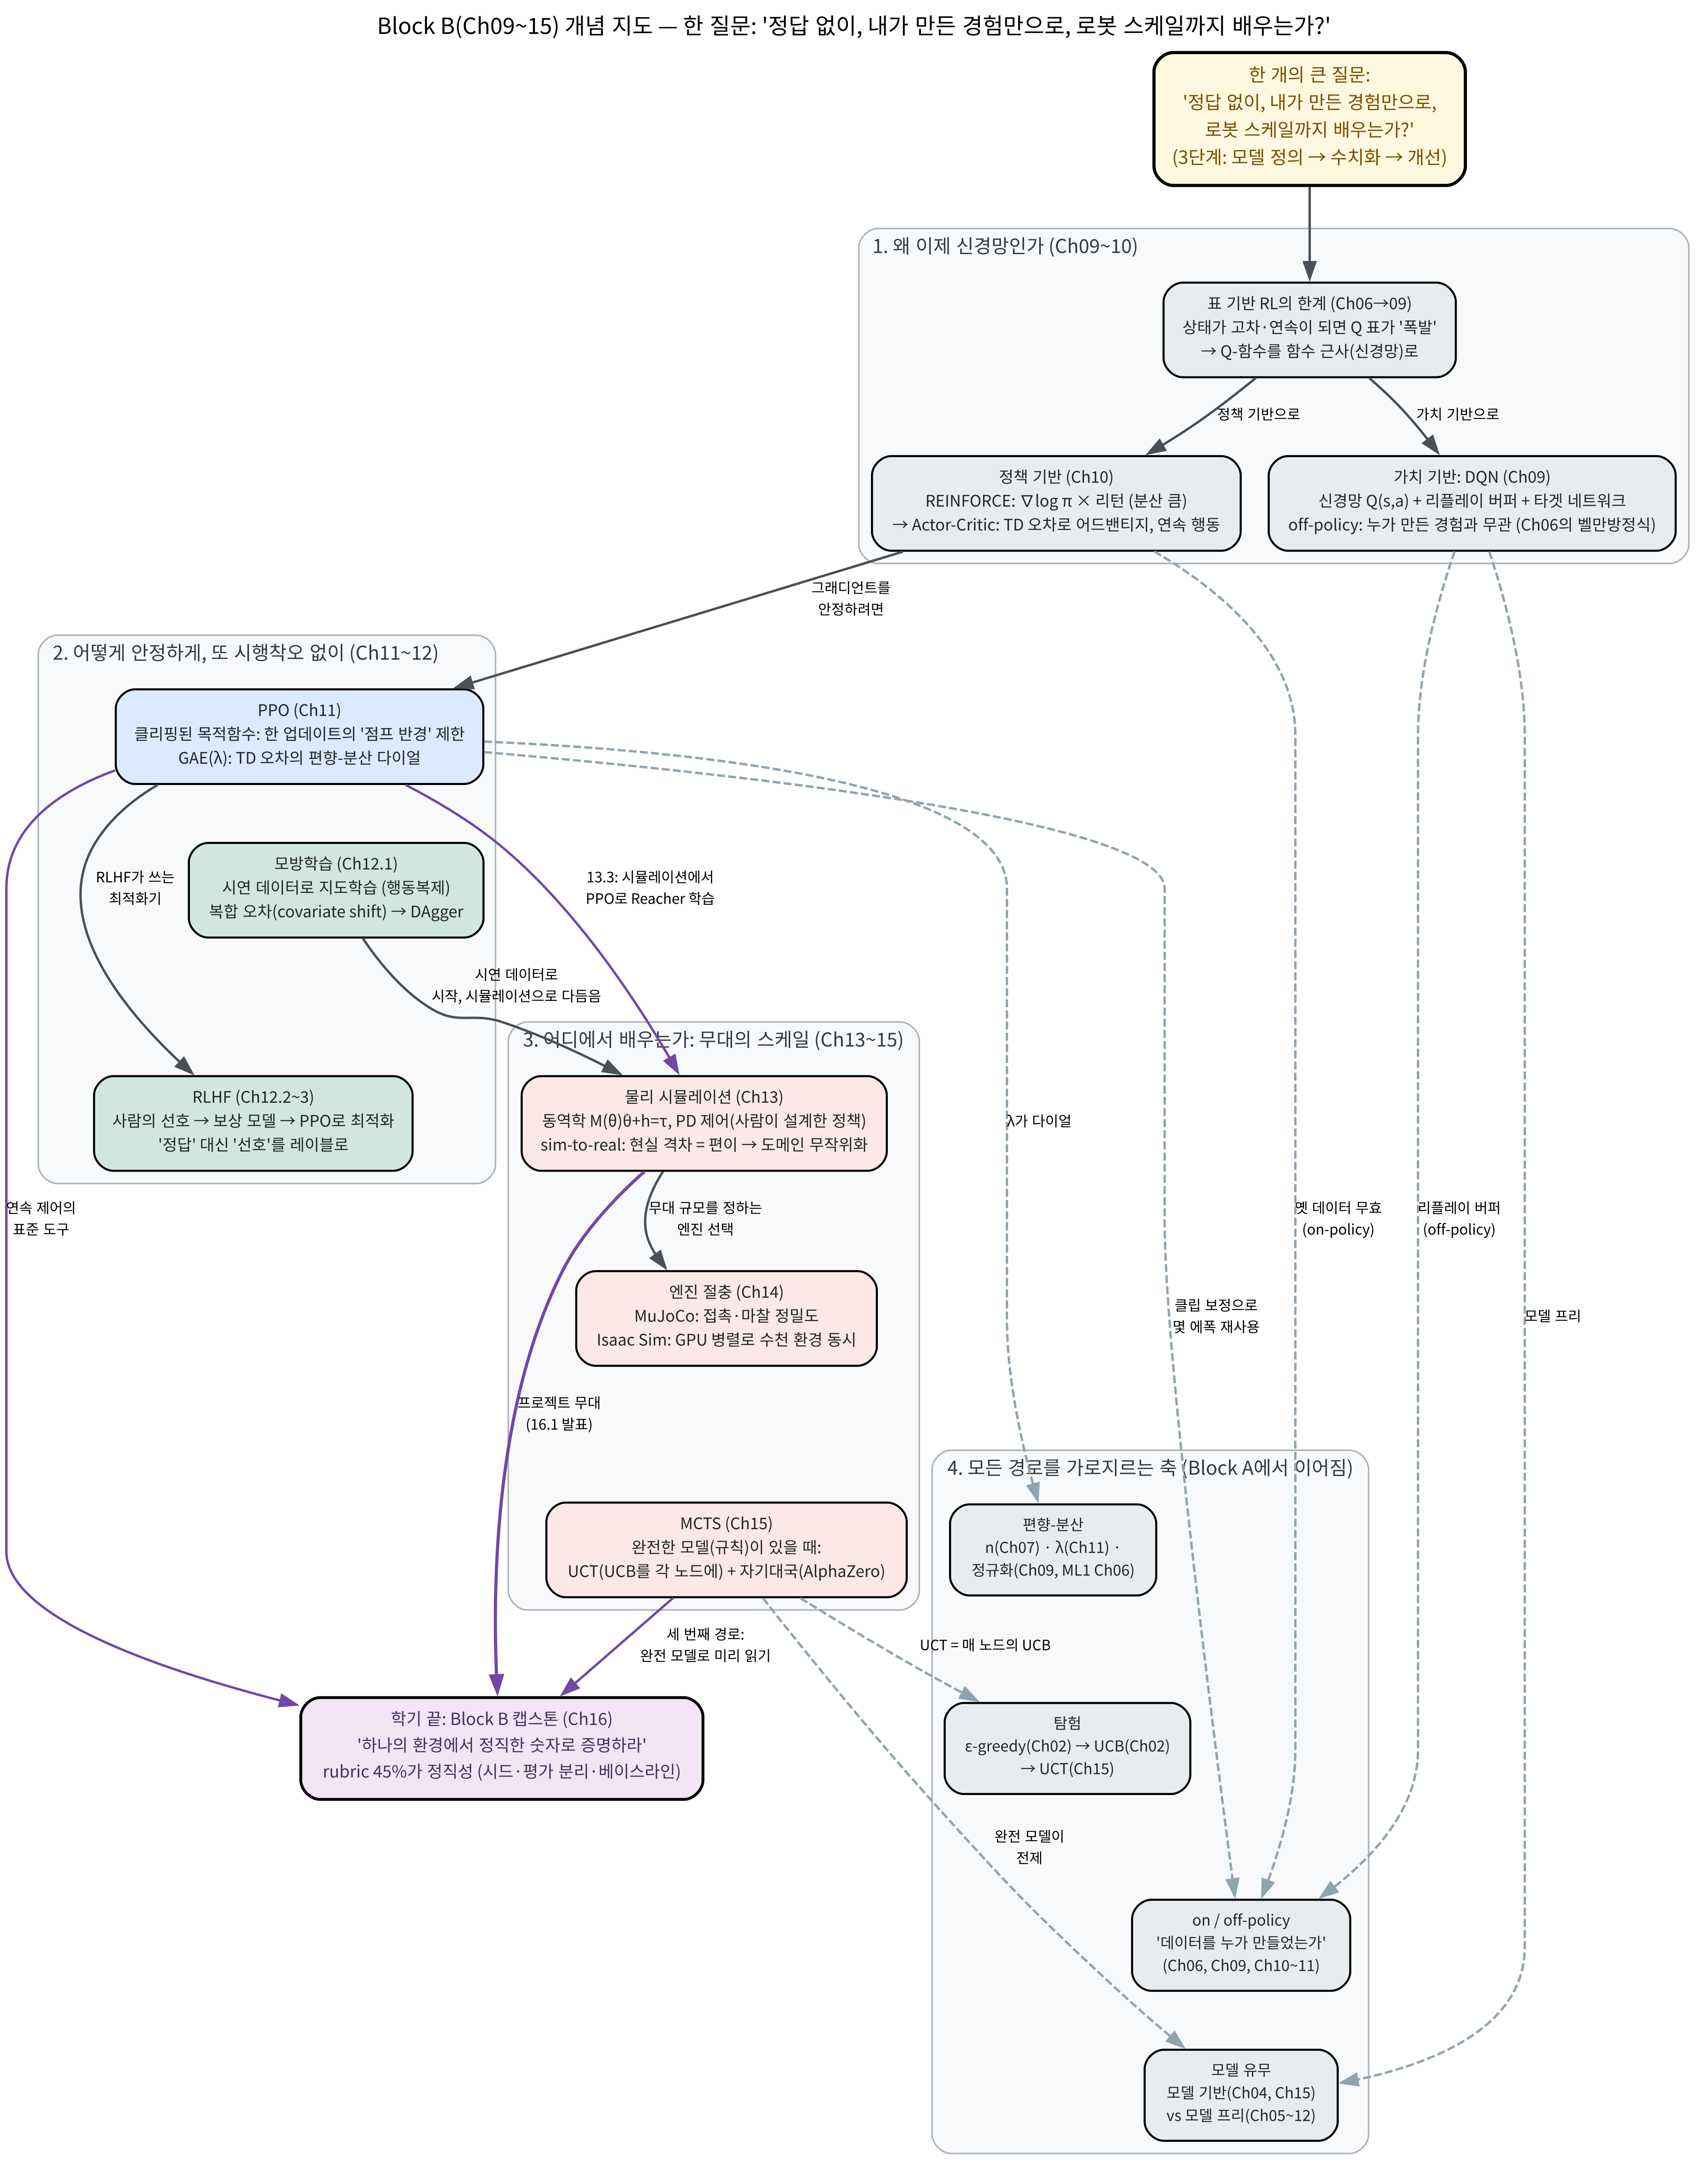
\includegraphics[width=\linewidth]{ch16_3_rl_concept_map.png}
      \vskip0.3em
      {\footnotesize 중앙: ``정답 없이, 내가 만든 경험만으로, 로봇
      스케일까지 배우는가''. 위: 왜 신경망인가(Ch9$\sim$10). 가운데:
      어떻게 안정하게(Ch11$\sim$12). 아래: 어디에서 배우는가(Ch13
      $\sim$15). 가로지르는 축: 편향-분산($\lambda, \varepsilon$),
      탐험($\varepsilon$-greedy $\to$ UCT), on/off-policy, 모델
      유무. 오른쪽: 학기 끝(16.1$\sim$16.3) — 하나의 환경에서 정직한
      숫자로 증명.}
    \end{column}
  \end{columns}
\end{frame}

\begin{frame}{확인 문제: 장을 넘나드는 복습 4개 (1)-(2)}
  \small
  \begin{itemize}
    \item \textbf{1.} Ch2.2의 \kb{UCB}와 Ch15.2의 \kb{UCT}는 수식이
      거의 똑같다. 무엇이 같고, 다른가?
      \vskip0.2em
      {\footnotesize $\to$ 둘 다 ``지금까지의 평균 성과 + 덜
      시도해본 정도에 대한 불확실성 보너스''라는 같은 형태
      ($\bar{X} + c\sqrt{\ln N / n}$). \textbf{다른 것은 적용 대상} —
      UCB는 \textbf{밴딧의 팔}(상태 없는 단일 선택) 하나하나에, UCT는
      \textbf{게임 트리의 매 노드마다} 독립적으로 적용되어 ``각 국면에서
      다음 수를 고르는'' 문제를 반복해서 푼다.}
    \item \textbf{2.} Ch6.1의 \kb{TD 오차}와 Ch10.3의
      \kb{Actor-Critic}은 어떤 관계인가?
      \vskip0.2em
      {\footnotesize $\to$ Actor-Critic의 \textbf{critic이 학습하는
      신호가 바로 TD 오차} — REINFORCE(10.2)가 에피소드 전체 리턴으로
      그래디언트 분산이 컸다면, AC는 그 리턴을 \textbf{TD 오차}(한
      스텝만 보고 계산한 어드밴티지 추정치)로 대체해 \textbf{분산을
      줄인다}. Ch11.3의 \textbf{GAE}는 이 TD 오차를 여러 스텝에
      걸쳐 지수가중평균한 \textbf{일반화}.}
  \end{itemize}
\end{frame}

\begin{frame}{확인 문제: 장을 넘나드는 복습 4개 (3)-(4)}
  \small
  \begin{itemize}
    \item \textbf{3.} DQN(off-policy)이 리플레이 버퍼의 \emph{오래된}
      경험을 재사용할 수 있는데, REINFORCE·PPO는 왜(
      \emph{PPO는 부분적으로만}) 그럴 수 없는가?
      \vskip0.2em
      {\footnotesize $\to$ DQN은 \textbf{Q-함수}(정답이 정해진 값)를
      배우는 것이라 ``누가 그 경험을 만들었는지''와 무관하게 벨만
      방정식이 성립 — \textbf{off-policy}. REINFORCE는 정책 그래디언트가
      ``\emph{지금} 정책이 그 행동을 선택할 확률''에 의존 — 정책이
      바뀌면 그 확률도 바뀌어 \textbf{옛 데이터의 그래디언트가 더 이상
      정확하지 않}다(\textbf{on-policy}). PPO는 확률비
      $r_t(\theta)$로 이 차이를 \textbf{보정}하고 클리핑으로 오차를
      억제해서 \emph{몇 에폭 정도}는 재사용 가능하지만, DQN처럼
      완전히 오래된 경험까지는 재사용 못 함.}
    \item \textbf{4.} Ch12.1 \kb{모방학습}(BC/DAgger)과 Ch15.2
      \kb{MCTS}는 둘 다 ``에이전트가 직접 시행착오를 겪는 것의
      대안''. 각각 무엇을 대신 활용하는가?
      \vskip0.2em
      {\footnotesize $\to$ 모방학습은 \textbf{사람의 시연}(전문가가
      실제로 어떻게 행동했는지)을 \textbf{정답} 삼아 지도학습으로
      정책을 배움. MCTS는 \textbf{완벽한 모델(규칙)로 만든 가상의
      시뮬레이션}을 반복해서, 실제로 행동하기 전에 결과를 미리
      들여다봄. 둘 다 표준 RL보다 \textbf{안전하거나 효율적}이지만,
      전자는 \textbf{사람의 시연 데이터}가, 후자는 \textbf{정확한
      모델(규칙)}이 있어야 한다는 \textbf{전제}가 필요.}
  \end{itemize}
\end{frame}

\begin{frame}{복습 자가진단 — 20문항}
  {\footnotesize 8.3의 20문항과 같은 형식 — 각 문항에 대해
  \textbf{10초 안에 한 문장으로} 답을 말할 수 있으면 O, 막히면 $\times$.
  18개 이상 = 준비 완료 / 15$\sim$17 = $\times$가 모인 장의 ``자주 하는
  실수''+확인 문제 다시 / 12$\sim$14 = §네 경로의 수식(TD 오차,
  클리핑된 목적함수)을 손으로 다시 유도 / 12 미만 = §자주 하는
  실수(총정리판)를 건너뛰지 않는다.}
  \vskip0.4em
  \scriptsize
  \begin{tabular}{@{}ll@{}}
    \toprule
    # & 한 문장 질문 (장) \\
    \midrule
    1 & DQN의 타겟 네트워크는 왜 매 스텝 갱신하면 안 되는가 (Ch09) \\
    2 & 리플레이 버퍼가 해결하는 문제와, DQN에서만 가능한 이유 (Ch09/06) \\
    3 & TD 오차를 $Q$로 표기하시오 (Ch06/09) \\
    4 & REINFORCE와 TD 갱신의 차이를 한 문장으로 (Ch10) \\
    5 & baseline 차분이 왜 편향을 만들지 않는가 (Ch10) \\
    6 & PPO의 클리핑이 막는 ``나쁜 일''은 무엇인가 (Ch11) \\
    7 & 정책 그래디언트가 왜 on-policy여야 하는가 (Ch10/11) \\
    8 & GAE의 $\lambda$가 0이면 / 1에 가까우면 각각 무엇이 되는가 (Ch11) \\
    9 & 행동복제가 ``복합 오차''로 나빠지는 메커니즘 (Ch12) \\
    10 & DAgger가 복합 오차를 피하는 방식 (Ch12) \\
    11 & RLHF에서 ``정답''이 아니라 무엇으로 레이블을 얻는가 (Ch12) \\
    12 & 로봇 정책을 시뮬레이션에서 학습하는 이유 두 가지 (Ch13) \\
    13 & 현실 격차가 ``잡음''이 아니라 ``편이''라는 말의 뜻 (Ch13) \\
    14 & 도메인 무작위화 범위가 넓은 것이 항상 좋은 것이 아닌 이유 (Ch13) \\
    15 & MuJoCo와 Isaac Sim의 트레이드오프를 한 문장으로 (Ch14) \\
    16 & AlphaZero가 정책망과 가치망을 \emph{둘 다} 쓴 이유 (Ch15) \\
    17 & UCT의 탐색 항이 ``시도 횟수''로 무엇을 쓰는지 (Ch15/02) \\
    18 & MCTS가 DP와 다른 점 — ``모델''을 어떻게 쓰는지 (Ch15/04) \\
    19 & 이번 학기 모든 알고리즘의 공통 3단계를 쓰시오 (전체) \\
    20 & ML1(지도학습)과 ML2(RL)의 가장 큰 차이를 한 문장으로 (전체) \\
    \bottomrule
  \end{tabular}
\end{frame}

\begin{frame}{자가진단 답 (한 줄) — 핵심 10문항}
  \scriptsize
  \begin{enumerate}
    \item \textbf{1} — 목표와 추정치가 서로를 따라다니며 발산하기
      때문(9.2절 보스팅 불안정의 방치 버전).
    \item \textbf{3} — $\delta = r + \gamma Q(s',a') - Q(s,a)$ —
      최적을 추구하면 $a'$ 자리에 $\max$.
    \item \textbf{5} — baseline $b(s)$가 $a$에 무관하므로
      $\mathbb{E}_a[\nabla \log \pi(a|s)\, b(s)] = b(s)\nabla
      \sum_a \pi(a|s) = 0$ — \textbf{분산만 줄고 편향은 0}.
    \item \textbf{6} — $r_t(\theta)$가 1에서 크게 벗어나 한
      업데이트에 정책이 ``멀리 점프''해 좋은 정책을 \textbf{망가뜨리는
      것} — 클리핑은 점프 반경을 제한.
    \item \textbf{8} — $\lambda=0$이면 TD(0)(편향 있음, 분산 작음),
      $\lambda\to 1$이면 (유한 에피소드에서) MC 리턴(편향 없음,
      분산 큼) — 7.2의 U자 스펙트럼.
    \item \textbf{9} — 전문가 데이터 \textbf{분포 밖} 상태에 들면 그
      행동이 신뢰 불가 $\to$ 다음 상태가 더 벗어난 분포로 $\to$
      오차가 \textbf{스텝마다 곱해짐}(covariate shift).
    \item \textbf{11} — 사람의 \textbf{선호}(두 응답 중 어느 것이
      나은지) — 선호 데이터로 \textbf{보상 모델}을 먼저 학습하고, 그
      보상으로 PPO.
    \item \textbf{13} — \textbf{systematic}한 차이이므로 시뮬레이션
      데이터를 늘려도 \textbf{사라지지 않}음 — ML1 Ch04
      bias-variance에서 ``편이는 데이터로 안 줄고''의 RL 버전.
    \item \textbf{15} — MuJoCo: 접촉·마찰 \textbf{정밀도}, Isaac: GPU
      \textbf{병렬화}(수천 환경 동시) — 정밀도 대 규모.
    \item \textbf{20} — ML1은 \emph{다른이(데이터 수집자)가 만든
      데이터와 정답}을 줘 맞히게 하고, ML2는 \emph{에이전트가
      행동해서 데이터를 스스로 만들고 정답 없이 보상만으로} 배운다 —
      ``\textbf{무엇을 데이터로 갖고, 무엇을 최적화하는가}''의
      답이 바뀌는 것.
  \end{enumerate}
\end{frame}

\begin{frame}{자주 하는 실수 — 총정리판}
  \small
  \begin{itemize}
    \item \textbf{``곡선이 올라갔다''로 ``왜 올라갔는지''를
      대체하기} — 16.1 좋은/나쁜 예의 학기 전체 버전. ``PPO로 학습
      했는데 리턴이 좋아졌다''는 문장은 Ch11의 어떤 개념도 \emph{사용}
      하지 않은 문장. ``보상 스케일링 1/8로 어드밴티지 분산이 줄었고
      (11.1), $\lambda=0.9$로 편향-분산 트레이드오프를 조정한(11.3)
      결과''까지가 한 문장이면, 그 팀은 이 학기를 \textbf{통과}한
      것.
    \item \textbf{``시뮬레이션에서 검증했다''로 ``완료'' 선언하기} —
      시뮬레이션 점수는 \textbf{시뮬레이션 환경의 점수}일 뿐, 시뮬
      상위권 정책이 \textbf{실물에서 꼴찌}로 뒤집힐 수 있음.
      물리 파라미터(감쇠, 마찰)를 넣었다면 그 파라미터를 바꿔 ``순위
      유지''가 성립하는지 확인한/안 한 팀의 점수가 rubric ``방법론
      적절성''에서 갈림.
    \item \textbf{``PPO가 더 좋았다''를 조건 없이 쓰기} — 알고리즘
      비교 결론에 \textbf{환경(연속/이산, 보상 구조), 시드 수,
      하이퍼파라미터}가 붙지 않으면 그 문장은 \textbf{무효}. 유효한
      버전: ``Pendulum, 시드 3개, 같은 총 스텝 수에서, PPO($\lambda
      =0.9$)가 REINFORCE 대비 에피소드당 리턴이 평균 12\% 높고 시드
      간 표준편차는 40\% 작았다''.
    \item \textbf{``수렴했다''와 ``좋다''를 혼동하기} — 탐험이
      부족한 상태의 Q값은 \emph{틀린 값으로 정확히} 수렴할 수 있고,
      곡선의 ``평탄화''는 수렴일 수도 \textbf{고착(stuck)}일 수도
      있음. 16.1 Pendulum 예($-1092$, 이론 최적과는 멀다) =
      ``개선됐지만 수렴한 것은 아니다''의 정직한 보고 예.
    \item \textbf{자기 프로젝트의 실패를 복습 자료로 안 쓰기} —
      ``이 실험의 이상한 결과를 원인으로 진단하라''형 질문(발표
      질의응답, 면접)에 답할 자료는 \textbf{바로 16.1의 ``잘 안
      됐던 부분과 원인 진단'' 절}. 자기 실험의 실패 한 건을
      \emph{개념으로 해석}한 능력은 어떤 참고서로도 대체 불가.
  \end{itemize}
\end{frame}

\begin{frame}{마지막 체크리스트 — 학기 이후에 가져갈 세 가지}
  {\footnotesize 공식 목록은 13개 장이지만, 졸업하고 몇 년 뒤에
  실제로 남는 것은 \textbf{세 가지}:}
  \vskip0.4em
  \begin{enumerate}
    \item \kb{``무엇을 데이터(경험)으로 갖고, 무엇을 최적화하고
      싶은가''라는 질문의 습관.} 새로운 문제(운영 전략, A/B 테스트,
      물리 설계, LLM 후학습)를 마주했을 때 ``어떤 에이전트·어떤
      보상·어떤 경험인가''로 \textbf{번역하는 연습}을 13번 한 것이
      이 학기. 알고리즘 이름은 잊어져도 \textbf{이 번역은 남는다} —
      ML1의 ``행의 단위, 정답의 유무''와 쌍을 이루는, 문제
      정식화 기술의 절반이 완성된 것.
    \item \kb{정직한 숫자에 대한 기준.} 시드 $\geq 3$ · 학습/평가
      분리 · 베이스라인 · ``완전히 수렴하지 않았다''는 문장 — 8.1
      에서 시작해 16.1에서 반복된 프로토콜의 정직성은, 강화학습만이
      아니라 \textbf{모든 실험 과학}(ML1 val/test 정직성과 같은
      뿌리)의 기본 문법.
    \item \kb{``같은 방정식, 다른 형태''의 지도.} 이 학기의 알고리즘
      13개는 \textbf{3단계 구조의 13가지 변주}에 불과 — 그래서 새
      알고리즘 논문을 만나도 ``이것은 ②번(수치화)을 바꾼 변주구나''
      에서부터 읽을 수 있다. 지도의 \textbf{엣지}를 말할 수 있는
      한, 지도는 \textbf{확장 가능한 자산}이고, \textbf{박스만}
      외운 한으로는 \textbf{재고}에 불과하다.
  \end{enumerate}
\end{frame}

\begin{frame}{최신 동향 — 이 학기가 이어지는 세 방향}
  {\footnotesize 이번 학기에서 다루기엔 이르지만 지금 활발히
  연구되는 방향 — ``지금 배운 것이 이런 곳으로 이어질 수 있다''는
  지도를 그리는 것이 목적.}
  \vskip0.4em
  \begin{itemize}
    \item \kb{오프라인 강화학습 (Offline RL)} — 환경과 직접
      상호작용하지 않고, \textbf{이미 모아둔 방대한 로그 데이터만으로}
      정책을 학습. 실물 로봇으로 탐험하는 것 자체가 위험하거나 비
      싼 상황(자율주행, 의료)에서 특히 중요. Ch12 모방학습과 문제의
      식이 비슷하지만, 시연이 아니라 \textbf{(좋은 것과 나쁜 것이
      섞인) 임의의 로그}로부터 배운다는 점이 다름.
    \item \kb{범용 로봇 정책 (Generalist Robot Policies)} — 하나의
      작업에 특화된 정책 대신, \textbf{다양한 로봇·작업에 걸쳐
      일반화되는 하나의 큰 정책}(RT-2, OpenVLA 등) — ML1의 \textbf{LLM
      사전학습} 아이디어를 로봇 제어에 적용한 것에 가까움: 방대한
      로봇 시연·상호작용 데이터로 폭넓게 학습한 뒤 특정 작업에
      맞게 다듬음.
    \item \kb{Sim-to-Real의 발전} — Ch13.1 도메인 무작위화를 넘어,
      \textbf{시뮬레이션과 실제 환경의 차이 자체를 학습으로
      메우려는} 연구 — Ch14 GPU 가속 시뮬레이션(Isaac Sim 등)이
      ``훨씬 많은 다양한 시뮬레이션 조건을 빠르게 경험시킨다''는
      방향으로 기여.
  \end{itemize}
  \vskip0.3em
  {\footnotesize \textbf{더 깊이} 파고들고 싶다면: 각 장에서
  ``이 학기 범위를 넘는다''고 언급됐던 부분 — TRPO의 상세 수학,
  DAgger의 수렴 증명, 멀티에이전트 RL의 내쉬 균형, AlphaZero의
  자기대국 학습 세부사항 등.}
\end{frame}

\begin{frame}{자주 묻는 질문 — 산출물·Block A/B 차이·다음 방향}
  \small
  \begin{itemize}
    \item \textbf{16.3의 산출물?} \textbf{두 개}: (1) §손으로
      한 번의 rubric 표 4행(``나쁠 때의 모습'' + ``시험하는
      질문''), (2) 20문항 자가진단에서 본인이 $\times$를 표한 것
      중 \textbf{3개}를 골라, 각각 ``말했어야 할 한 줄''을
      \textbf{자기 언어로} 쓰는 것. $\times$ 개수 자체는 점수가
      \textbf{아니다} — $\times$를 \emph{자기 언어로 메운 문장}이
      점수화. 16.1 = ``프로젝트를 정직하게 수행했는가'', 16.2 =
      ``남의 프로젝트를 구체적으로 심사를 했는가'', 16.3 = ``\textbf{학기
      전체를 자기 것으로 만들었는가}''를 묻는 블록.
    \item \textbf{Block A vs Block B 복습은 어디에 시간을?}
      요구사항의 \textbf{형태}가 바뀌었다 — Block A: ``알고리즘
      최소 2개 비교'' + 개념 연결 / Block B: \textbf{알고리즘 1개
      + 수식적 정당화 1개}. ``어떤 알고리즘을 썼는가''보다
      \textbf{``왜'' 그 하이퍼파라미터(보상 스케일, $\gamma,
      \lambda$, 클립 $\epsilon$)를 그렇게 골랐는가}가 점수의 대부분을
      결정 — 복습의 무게중심도 ``개념 나열''에서 \textbf{``개념
      $\to$ 내 실험의 숫자''를 잇는} 연습으로 이동.
    \item \textbf{졸업 후 자연스러운 다음은?} §최신 동향의
      \textbf{세 방향}이 현재 주류 — 오프라인 RL(로그 데이터만
      있는 실서비스), 범용 로봇 정책(LLM 사전학습이 로봇으로
      건너간 지점), Sim-to-Real(13$\sim$14장의 정면 돌파).
      공통 지름줄은 \textbf{하나}: 3단계 구조(모델 정의 $\to$
      수치화 $\to$ 개선)로 그 연구를 \textbf{자신만의 언어로
      다시 정식화}할 수 있는가.
  \end{itemize}
\end{frame}

\begin{frame}{마지막 한 문장}
  \begin{center}
    \large
    ML1이 ``\textbf{정답이 있는 데이터}로부터 배운다''는 세계였다면,\\
    ML2는 ``\textbf{스스로 행동해서 얻은 경험}만으로 배운다''는
    \textbf{완전히 다른 세계}.
  \end{center}
  \vskip0.8em
  \begin{itemize}
    \item \kb{밴딧}의 탐험-활용 딜레마에서 시작해 \kb{MDP} ·
      \kb{동적계획법} · \kb{몬테카를로} · \kb{시간차 학습}으로
      이론을 다졌고, \kb{신경망}과 결합해 그 이론을 \textbf{로봇
      시뮬레이션}이라는 현실적인 무대까지 끌고 왔다.
    \item 이제 이 두 세계 모두에서, \kq{``무엇을 데이터(또는
      경험)로 갖고 있고, 무엇을 최적화하고 싶은가''}라는 \textbf{같은
      질문}을 던질 수 있을 것이다.
  \end{itemize}
\end{frame}

% ===== wrap-up =====
\begin{frame}{이번 주차 정리}
  \small
  \begin{itemize}
    \item \kb{16.1 팀 프로젝트: 발표} — \textbf{환경}은
      ``개념 X가 돋보이는 \textbf{무대}'' 기준으로, 알고리즘과
      \textbf{페어링}. \textbf{베이스라인}(무작위 $-1274$, zero-torque
      $-1230$)을 \textbf{먼저} 재야 ``개선''의 방향을 말할 수 있다.
      \textbf{$\varepsilon=0$의 대응물 = $a=\mu$ 결정적 평가}
      ($\sigma$는 학습된 파라미터라 0으로 \emph{바꾸지 않고},
      샘플링만 안 함). 12만 스텝 Pendulum 실습: 학습 도중 마지막
      10($-673/-732/-668$)이 베이스라인 2배여도, \textbf{결정적
      평가($\approx-1403$)가 베이스라인($-1274$) \emph{아래}} —
      ``곡선이 올랐다'' $\neq$ ``무작위보다 낫다''. M2에
      \textbf{학습 예산 추정}(22초 기준선). \textbf{수식적
      정당화} = 수치 + ``완전 수렴 아님''의 정직함 + 하이퍼파라미터
      근거. \textbf{채점 = 정직성 45\%} — 프로토콜 정직성이
      정책의 질보다 중요.
    \item \kb{16.2 Peer-Review} — \textbf{역전}의 주: 네가
      심사위원. 5항목(환경/알고리즘 선택/정당화/정직성/탐험-활용)
      + \textbf{1점(감상평) $\to$ 2점(일반 지적) $\to$ 3점(반박
      가능한 질문 = 개념 명시 + \textbf{답이 나쁘면 결과가
      흔들림})}. 신경망 특유의 \textbf{``우연히 좋은'' 패턴 5가지}:
      시드 1개 학습 곡선, 학습 도중 리턴으로 수렴 결론,
      하이퍼파라미터 ``적당히'', 이산용( DQN)을 연속에,
      베이스라인 없이 ``잘 배웠다''. 실습: 가상 발표(시드 42,
      $-742.0$)를 재실행 — 같은 정책, 다른 프로토콜로 $-742$
      vs $-1413/-1491$(결정론적), 무작위 $-1239$ \textbf{아래}로
      뒤집힘. 시드 간 sd(약 70) $>$ 개선폭(약 63). \textbf{발표
      전 셀프-리뷰}가 최선의 전략.
    \item \kb{16.3 ML2 총정리} — \textbf{새로운 개념 없음}. 하나의
      MDP(달리거나 쉬거나, $\gamma=0.9$)를 \textbf{네 경로}로:
      ① DP $V^*(S)=2.589$(정확) / ② MC 2.594(편향 없음) / ③
      SARSA \textbf{2.29}(행동 정책 $V^\pi$, 간극 0.297 =
      ``탐험의 가격'') / ④ Q-learning 2.64($\max$ 한 줄이
      \textbf{수렴 대상 자체}를 변경). \textbf{두 과목을 관통하는
      3단계}: 모델 정의 $\to$ 틀린 정도 수치화 $\to$ 개선.
      개념 지도 읽기: \textbf{질문은 박스와 축의 교차점(엣지)},
      엣지가 곧 ``왜''. 20문항 자가진단 + ``학기 이후에 가져갈
      세 가지''(번역의 습관 · 정직한 숫자의 기준 · ``같은
      방정식, 다른 형태''의 지도). 최신 동향: \textbf{오프라인
      RL · 범용 로봇 정책(RT-2/OpenVLA) · Sim-to-Real}.
  \end{itemize}
  \vskip0.5em
  \begin{block}{이 학기의 마지막 문장}
    ML1 = ``정답이 있는 데이터로부터'', ML2 = ``\textbf{스스로
    행동해서 얻은 경험}만으로''. 이제 두 세계 모두에서 ``무엇을
    데이터(경험)로 갖고, 무엇을 최적화하고 싶은가''를 던질 수
    있다.
  \end{block}
\end{frame}

\end{document}
